\documentclass[frenchb]{article}
\usepackage[utf8]{inputenc}

\usepackage{graphicx}
\usepackage{color}

\usepackage{geometry}
\geometry{hmargin=2.5cm,vmargin=1.5cm}


\usepackage[T1]{fontenc}
\usepackage{a4wide}
\usepackage{graphicx}
\usepackage{amssymb}
\usepackage{amsmath}
\usepackage{color}
\usepackage{babel}
\usepackage{mathtools}

\begin{document}

\begin{figure}[t]
\centering

\includegraphics[width=5cm]{inp_n7.png}
\end{figure}

\title{\vspace{4cm} \textbf{Étude de chaînes de transmission en bande de base}}
\author{Nom des auteurs\\ \textsc{Cazes} Noa\\ \textsc{Martin} Cédric}
\date{\vspace{11cm} Département Sciences du Numérique - Première année \\
2019-2020 }

\maketitle

\newpage
\tableofcontents
\listoffigures

\newpage
%%%%%%%%%%%%%%%%%%%%%%%%%%%%%%%%%%%%%%%%%%%%%%%%%%%%%%%%%%%%%%%%%%
\section{Introduction}
%%%%%%%%%%%%%%%%%%%%%%%%%%%%%%%%%%%%%%%%%%%%%%%%%%%%%%%%%%%%%%%%%%
\subsection{Objectifs du travail réalisé}
L'étude réalisée a comme objectif de comparer l'influence du filtre de mise en forme, du filtre de récéption, de la transmission à travers un canal, et du nombre de symboles ($M$ dans un mapping $M-aire$) sur l'efficacité spectrale et en puissance de la chaîne considérée.

La comparaison est faite par rapport à une chaîne dite de réference, dont le filtre de réception et le filtre de mise en forme sont des filtres causaux rectangulaires de longueur $T_s$ (durée symbole), et avec un mapping $2-aire$.

\subsection{Schéma général des chaines à étudier (canal AWGN)}
La figure \ref{chaine_ex1} présente le schéma général des chaines à étudier.

\begin{figure}[ht!]
\centering
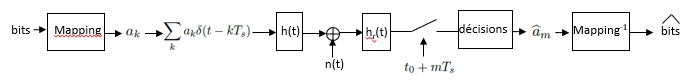
\includegraphics[width=15cm]{figure1.png}
\caption{Chaîne de transmission en bande de base}.
\label{chaine_ex1}
\end{figure}

\subsubsection{Génération de l'information binaire à transmettre}
La génération de l'information binaire à transmettre (bits $0$ et $1$ équiprobables et indépendants) pourra être réalisée grâce à la fonction \emph{randi} de Matlab.
%Mais ses éléments peuvent aussi provenir d'un texte ou d'une image.\\
%Pour associer une information binaire à un texte (et un texte à une information binaire), vous pouvez, par exemple, utiliser les lignes de code matlab suivantes :
%\begin{itemize}
%\item Bits=double(str2bin('Texte')).';
%\item ...
%\item TexteRecu=bin2str(BitsRecus);
%\end{itemize}
%
%Pour associer une information binaire à une image noir et blanc (et une image noir et blanc à une information binaire), vous pouvez, par exemple, utiliser les lignes de code matlab suivantes :
%\begin{itemize}
%\item Image = imread('barbara.png');
%\item ImageBinaire=de$2$bi(Image);
%\item VecteurBinaire=double(reshape(ImageBinaire.',$1$,size(ImageBinaire,$1$)*size(ImageBinaire,$2$)));
%\item ...
%\item xx=reshape(BitsRecus,size(ImageBinaire,$2$),size(ImageBinaire,$1$));
%\item ImageRecue=reshape(bi$2$de(xx.'),size(Image,1),length(xx)/size(Image,$1$));
%\item figure; imagesc(ImageRecue); colormap('gray');
%\end{itemize}

%Remarque : afin de les rendre indépendants, lorsqu'ils proviennent d'un texte ou d'une image, il peut être nécessaire d'embrouiller les bits représentant l'information à transmettre.

\subsubsection{Mapping}
Un mapping devra être réalisé afin de passer de l'information binaire aux symboles $a_k$. Le mapping est un des élements qui pourra différer selon les chaines de transmission à étudier et implanter.

\subsubsection{Suréchantillonnage}
La suite d'impulsions de Dirac espacées de la durée symbole $T_s$ et pondérées par les symboles $a_k$ issus du mapping sera générée, en numérique, en insérant $N_s-1$ zéros entre deux symboles $a_k$, si $N_s$ représente le nombre d'échantillons utilisés par symbole (ou facteur de suréchantillonnage : $T_s=N_sT_e$, $T_e$ étant la période d'échantillonnage). $N_s$ devra être déterminé pour que le signal numérique généré respecte la condition d'échantillonnage de Shannon.

\subsubsection{Filtrage de mise en forme}
La réponse impulsionnelle, $h(t)$, du filtre de mise en forme est un des élements qui pourra différer selon les chaines de transmission à étudier et implanter. Ne seront implantés que des filtres de type RIF (à réponse impulsionnelle finie). Une fois la réponse impulsionnelle numérique générée ($h=\left[h(0) h(1) ... h(N-1)\right]$, si $N$ représente l'ordre du filtre), le filtrage pourra être réalisé en utilisant la fonction \emph{filter} de matlab : \emph{signal$\_$filtre=filter($h$,$1$,signal$\_$a$\_$filtrer)} (attention alors au retard dû à la causalité du filtre) ou bien en utilisant la fonction \emph{conv.m}, comme lors des TPs de traitement du signal.

\subsubsection{Canal de transmission AWGN}
Le canal de transmission est supposé à bruit, $n(t)$, additif blanc et Gaussien, de densité spectrale de puissance égale à $\frac{N_0}{2}$ quelle que soit la fréquence. Pour les simulations, ce bruit sera généré sur la bande $F_e$ (fréquence d'échantillonnage), grâce à la fonction randn de matlab, avec plusieurs puissances différentes, notées $\sigma_n^2$ : $bruit=\sigma_n \ast randn(1,length(r));$, si $r$ représente le vecteur d'échantillons de signal à l'entrée du récepteur. On calculera la puissance du bruit $\sigma_n^2$, en fonction des rapports signal à bruit par bit souhaités à l'entrée du récepteur $\frac{E_b}{N_0}$, de la manière suivante (voir démonstration en annexe):
$$
\sigma_n^2=\frac{P_r N_s}{2 \log_2(M) \frac{E_b}{N_0}},
$$
où $N_s$ représente le facteur de suréchantillonage, $M$ l'ordre de la modulation et $P_r$ la puissance du signal $r$ qui peut être obtenue sous matlab de la manière suivante : $P_r=mean(abs(r). \; \hat{ }\;2)$.

\subsubsection{Filtrage de réception}
La réponse impulsionnelle, $h_r(t)$, du filtre de mise de réception est un des élements qui pourra différer selon les chaines de transmission à étudier et impanter. Ne seront implantés que des filtres de type RIF (à réponse impulsionnelle finie). Une fois la réponse impulsionnelle numérique générée ($hr=\left[hr(0) hr(1) ... hr(N-1)\right]$, si $N$ représente l'ordre du filtre), le filtrage pourra être réalisé en utilisant la fonction \emph{filter} de matlab : \emph{signal$\_$filtre=filter($hr$,$1$,signal$\_$a$\_$filtrer)} (attention alors au retard dû à la causalité du filtre) ou bien en utilisant la fonction \emph{conv.m}, comme lors des TPs de traitement du signal.

\subsubsection{Echantillonnage}
Le signal filtré devra être échantillonné à $t_0+mT_s$ pour revenir au rythme symbole. L'instant d'échantillonnage optimal $t_0$ pourra être déterminé dans l'étude théorique de la chaine à implanter et retrouvé grâce au tracé d'un diagramme de l'oeil sans bruit en sortie du filtre de réception.

\subsubsection{Décisions}
Un détecteur à seuil permettra de prendre les décisions sur les symboles à partir du signal échantillonné. Le seuil optimal devra être déterminé dans l'étude théorique de la chaine à implanter et retrouvé grâce au tracé d'un diagramme de l'oeil sans bruit en sortie du filtre de réception.

\subsubsection{Demapping} Un demapping devra être réalisé en vue de comparer les bits reçus aux bits émis dans l'objectif de calculer le taux d'erreur binaire simulé de la transmission, TEB simulé qui devra être comparé au TEB théorique déterminé dans l'étude théorique de la chaine en question.\\


%%%%%%%%%%%%%%%%%%%%%%%%%%%%%%%%%%%%%%%%%%%%%%%%%%%%%%%%%%%%%%%%%%
\section{Première chaine à étudier : "chaine de référence"}
%%%%%%%%%%%%%%%%%%%%%%%%%%%%%%%%%%%%%%%%%%%%%%%%%%%%%%%%%%%%%%%%%%
On considèrera un mapping binaire à moyenne nulle (symboles $a_k \in \left\{-1,1\right\}$) et des réponses impulsionnelles des filtres de mise en forme et de réception, $h(t)$ et $h_r(t)$, rectangulaires de durée $T_s$. Le résultat du produit de convolution entre $h(t)$ et $h_r(t)$ est donné dans la figure \ref{prod_conv1}.

\begin{figure}[ht!]
\centering
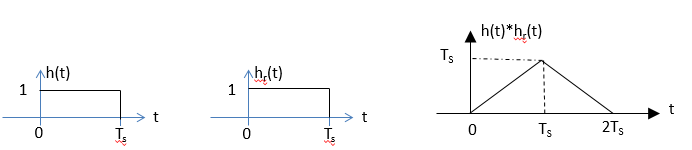
\includegraphics[width=10cm]{figure2.png}
\caption{Produit de convolution entre $h(t)$ et $h_r(t)$.\label{fig : prod_conv1}}
\end{figure}

\newpage
\subsection{Etude théorique}

    \begin{enumerate}
        \item Calculer la densité spectrale de puissance (DSP) du signal transmis. Quelle est, en théorie, la bande nécessaire à la transmission d'un tel signal ?
        \par\leavevmode\par
        \setlength\parindent{0.5cm}
        Comme le mapping est à moyenne nulle et que, par hypothèse, les symboles sont indépendants:
        
        \begin{equation*}
        \begin{split}
        \forall k \ne 0, R_a(k) &= 0 \\
        \sigma_a^2 &= 1 \\
        S(f) &= \frac{1}{T_s} |H(f)|^2 \\
        S(f) & = T_s \ sinc^2(\pi f T_s) \\
        \end{split}
        \end{equation*}
        
        En théorie, la bande nécessaire à la transmission est de $\frac{2}{T_s}$ (entre $- \frac{1}{T_s}$ et $\frac{1}{T_s}$). 
        
        \item La chaîne de communication peut-elle vérifier le critère de Nyquist ? Justifiez votre réponse.
        \par\leavevmode\par
        \setlength\parindent{0.5cm}
        Le critère de Nyquist en temporel est tel que: 
        \begin{equation*}
        \begin{split}
        \exists t_0 \; \forall l \ne 0 & \; g(t_0 + l T_s) = 0 \\   
        g(t_0) & \ne 0 \\
        \end{split}
        \end{equation*}
        
        \setlength\parindent{0.5cm}
        D'après la figure \ref{fig : prod_conv1}, on considère:
        $$ \boxed{t_0 = T_s} $$
        $$ g(t_0)     = T_s  $$ 
        \item Sans bruit, tracer le signal $z(t)$ en sortie du filtre de réception $h_r(t)$ pour la suite de bits émise suivante : $0110100$. Retrouve-t-on sur ce signal le fait que la chaine de transmission puisse respecter le critère de Nyquist ?
        
        \begin{figure}[ht!]
		\centering
		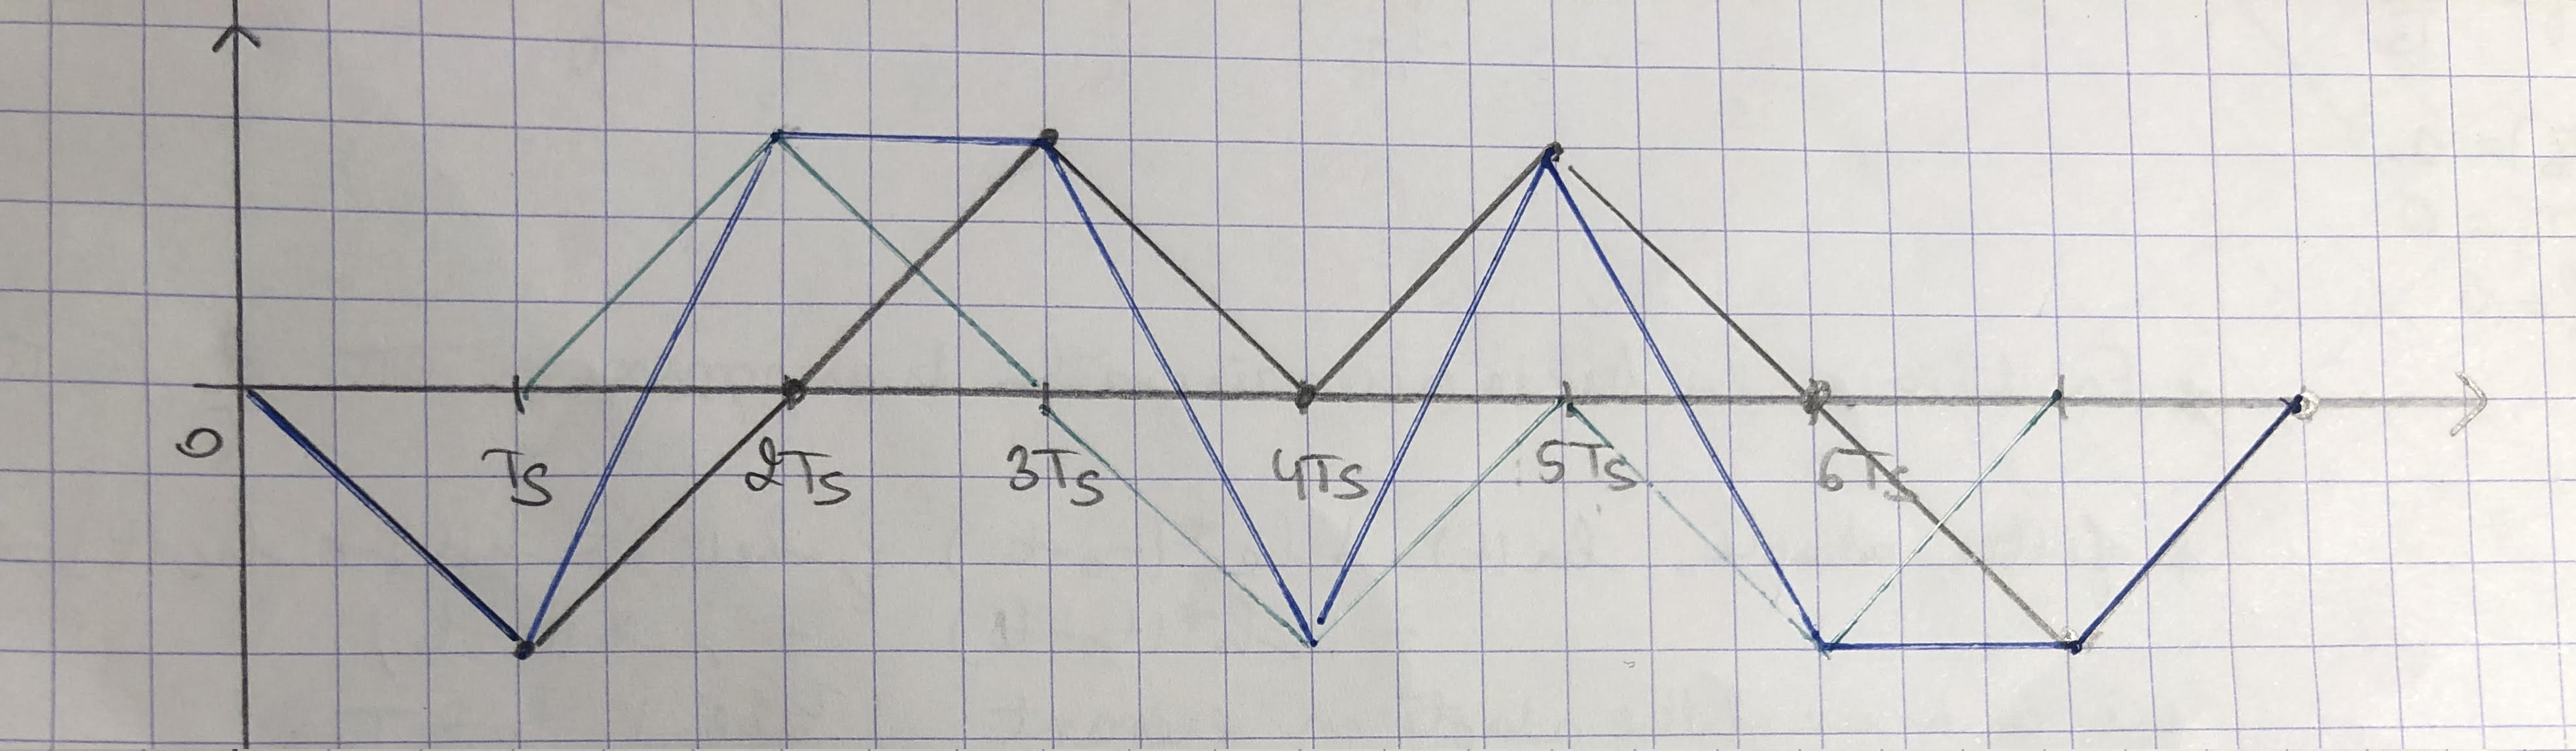
\includegraphics[width=10cm]{C1Q3.jpg}		\caption{Signal $z(t)$ en sortie du filtre de réception $h_r(t)$ pour $0110100$. \label{fig : C1Q3}}
		\end{figure}

        \par\leavevmode\par
        \setlength\parindent{0.5cm}
        Sur la figure \ref{fig : C1Q3}, on voit qu'il n'est pas évident de retrouver à première vue que le critère de Nyquist est respecté. 
        \par\leavevmode\par
        \item Toujours sans bruit, tracer le diagramme de l'oeil avec une base de temps de $T_s$. Retrouve-t-on sur le diagramme de l'oeil le fait que la chaine de transmission puisse respecter le critère de Nyquist ?
        
        \begin{figure}[ht!]
		\centering
		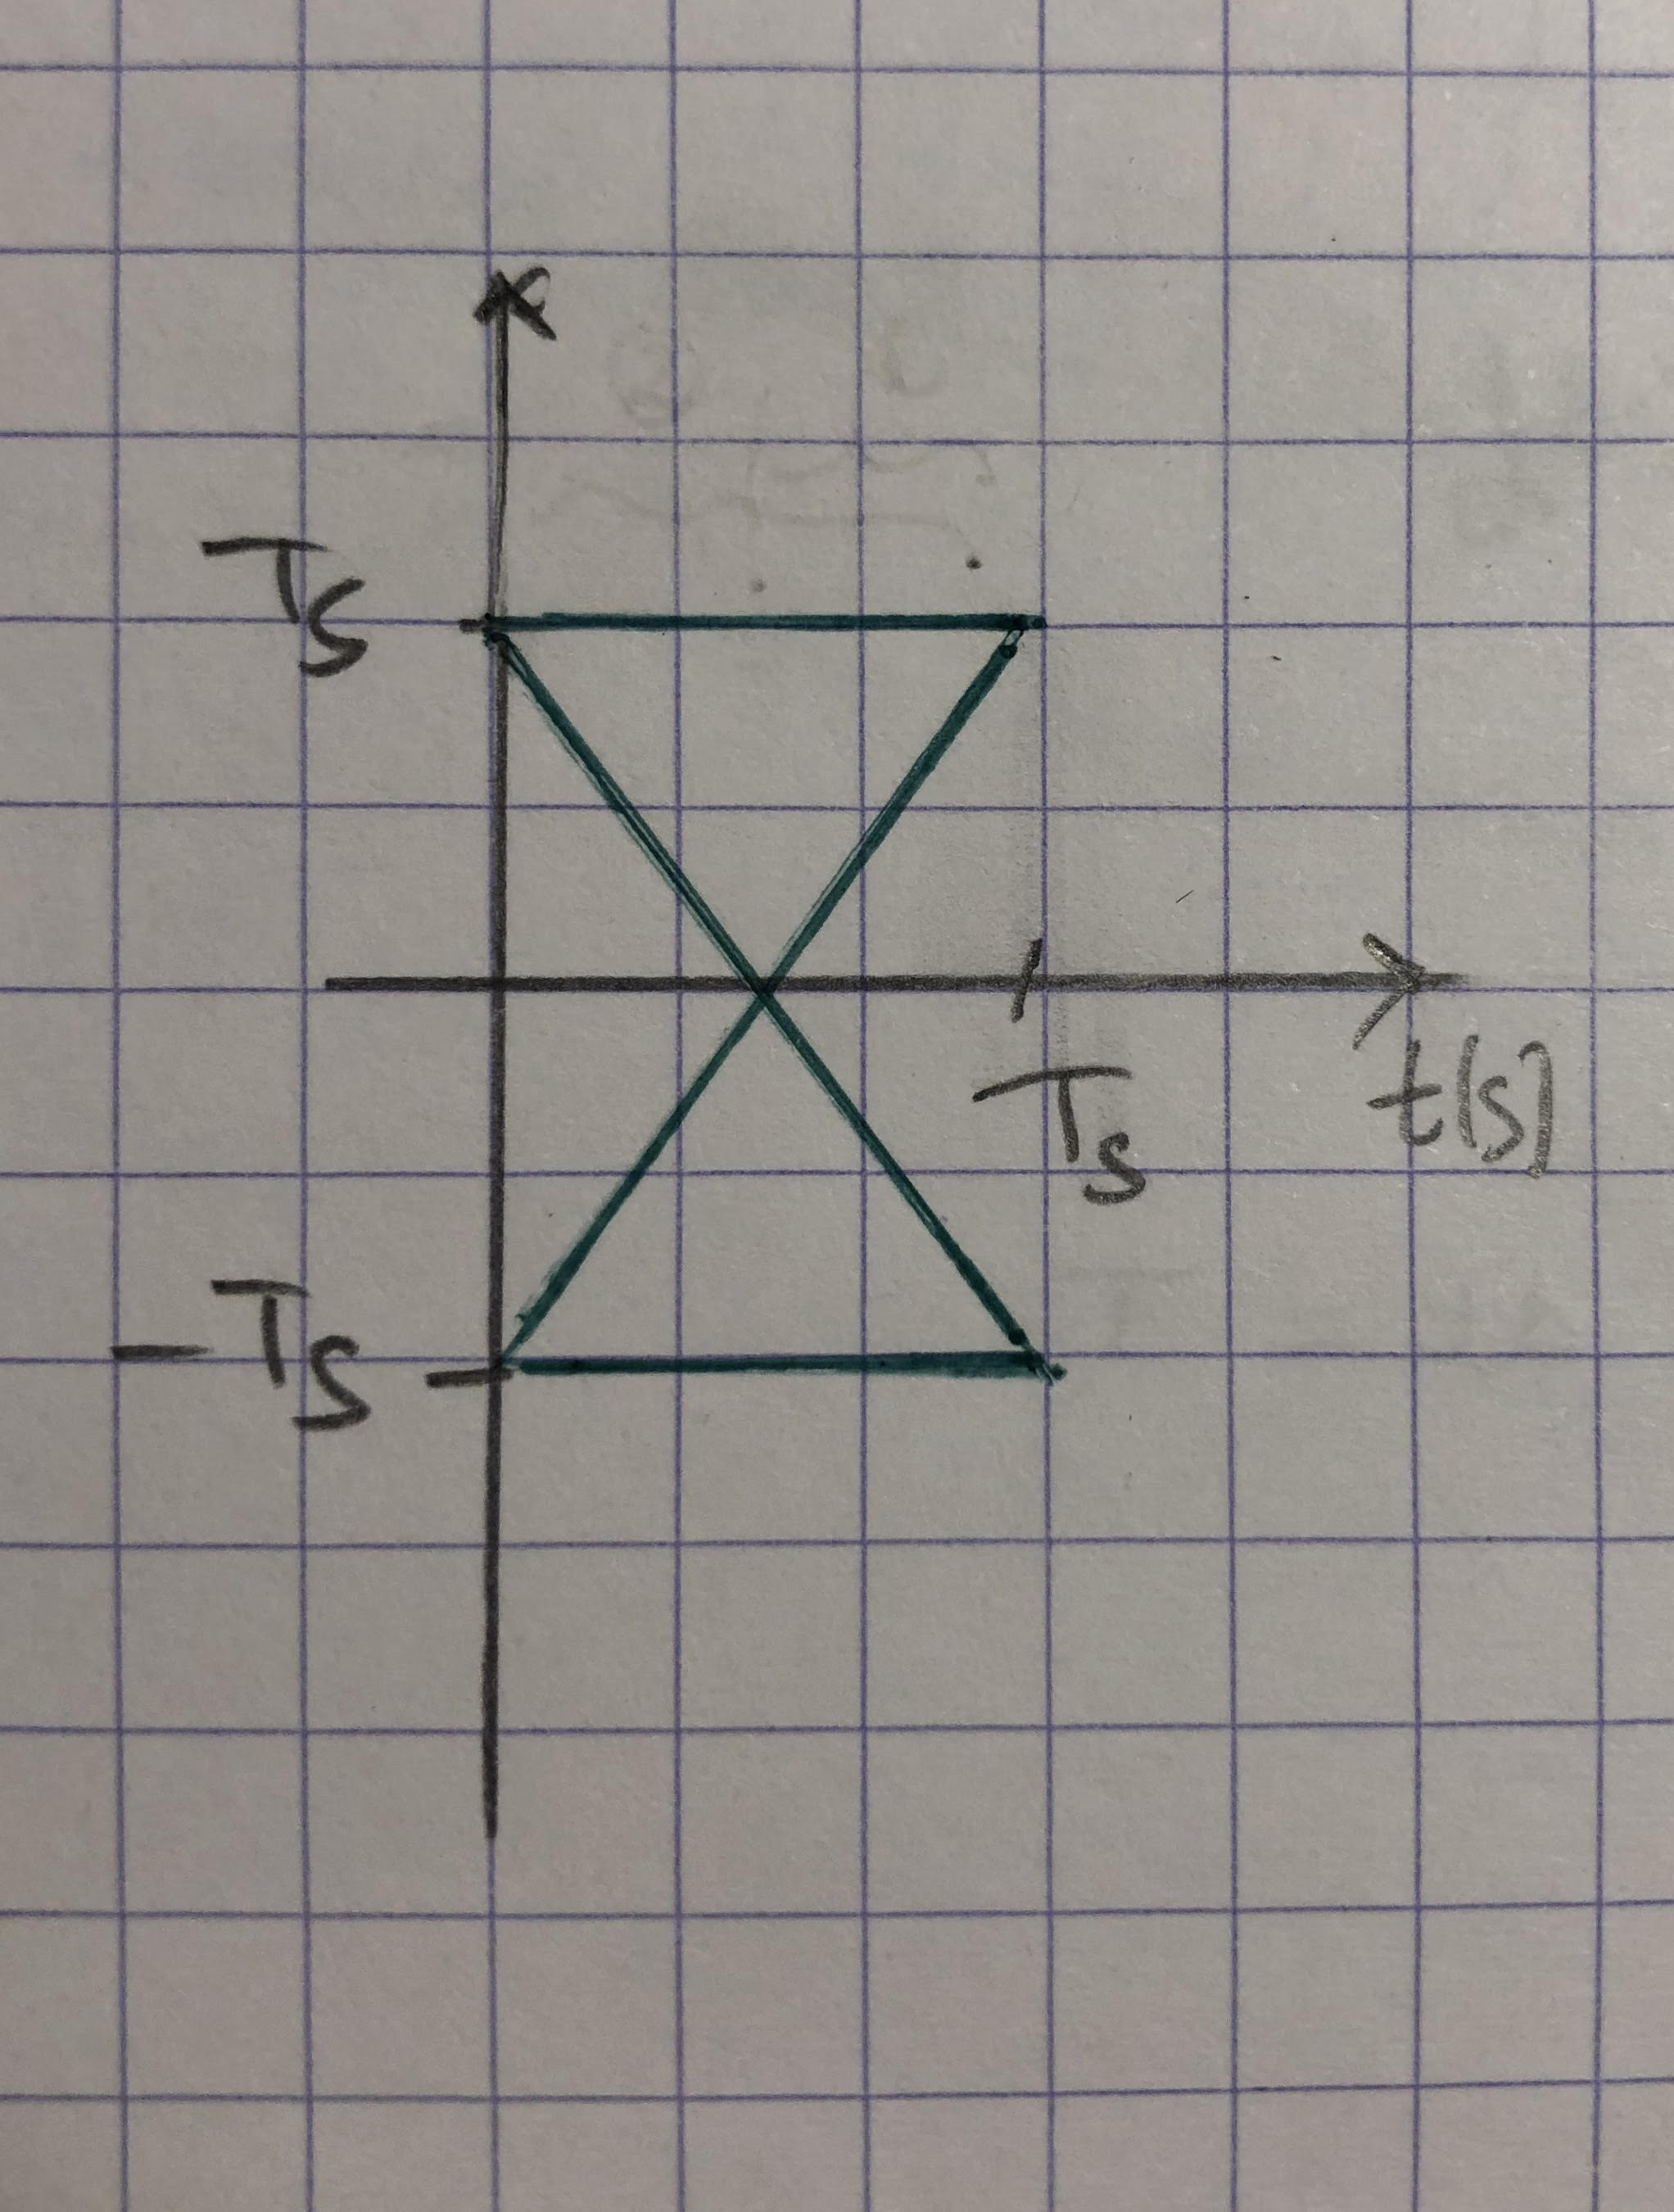
\includegraphics[width=5cm]{C1Q4.jpg}		\caption{Diagramme de l'oeil. \label{fig : C1Q4}}
		\end{figure}

        \par\leavevmode\par
        \setlength\parindent{0.5cm}
        Sur la figure \ref{fig : C1Q4}, on voit ici que le critère de Nyquist est réspecté pour $t_0 = T_s$.
         \par\leavevmode\par
        \item En supposant que l'on échantillonne aux instants optimaux (sans ISI), calculer le rapport signal sur bruit aux instants d'échantillonnage (on admettra que la puissance du bruit échantillonné et filtré est identique à celle du bruit filtré et on calculera donc cette puissance en sortie du filtre de réception).
        
        \begin{equation*}
        \begin{split}
        SNR & = \frac{P_s}{\sigma^2} \\        
        z_m &= a_m g(t_0)\\
        z_m & = a_m T_s\\
        P_s & = \mathbb{E}\left(\left(a_m T_s\right)^2\right) \\
        P_s & = \mathbb{E}\left(T_s^2\right) \\
        P_s & = T_s^2 \\
        \end{split}
        \end{equation*}
         
        D'après la définition de la puissance du bruit:
        
        \begin{equation*}
        \begin{split}
        P_{\omega} &= \int_\mathbb{R}S_{\omega}(f) \ \mathrm{d}f \\
        \end{split}
        \end{equation*}
        
        D'après la formule de Wiener-Lee:
        
        \begin{equation*}
        \begin{split}
        P_{\omega} = \int_{\mathbb{R}}|H_r(f)|^2 \frac{N_0}{2} \ \mathrm{d}f \\
        \end{split}
        \end{equation*}
        
        D'après notammant l'égalité de Parseval, on en déduit: 
        \begin{equation*}
        \begin{split}
        \sigma = \sqrt{\frac{N_0 T_s}{2}}  \\
        \end{split}
        \end{equation*}
        
        Donc: 
        \begin{equation*}
        \begin{split}
        \boxed{SNR = \frac{2 T_s}{N_0}}  \\
        \end{split}
        \end{equation*}
        \par\leavevmode\par
        \item On choisira d'utiliser un détecteur à seuil. Déterminer le seuil optimal à utiliser en expliquant votre choix.
        \par\leavevmode\par
        \setlength\parindent{0.5cm}
        On choisit 0 comme seuil, car on dispose d'une gaussienne centrée sur $T_s$ et d'une autre gaussienne centrée sur $- T_s$.
        \par\leavevmode\par
        \item En supposant que l'on échantillonne aux instants optimaux et que l'on utilise le seuil optimal de décision, donner le taux d'erreur binaire de la transmission en fonction de $T_s$ et $\sigma$, $\sigma^2$ représentant la puissance du bruit en sortie du filtre de réception $h_r(t)$.
        
        \par\leavevmode\par
        \setlength\parindent{0.5cm}
        Comme on a un mapping binaire: 
        \begin{equation*}
        \begin{split}
        nb_{symboles faux} &= nb_{bits faux} \\
        TES & = TEB \ log2(M)\\
        TES & = TEB \\
        \end{split}
        \end{equation*}
        
        Comme on respecte le critère de Nyquist et que le filtre de réception est un filtre adapté:
        
        \begin{equation*}
        \begin{split}
        TES & = Q\left(\frac{V g(t_0)}{\sigma} \right) \\
        TES & = Q\left(\frac{T_s}{\sigma} \right) \\ 
        \end{split}
        \end{equation*}
        
        Donc: 
        $$\boxed{ TEB = Q\left(\frac{T_s}{\sigma} \right)}$$
        \par\leavevmode\par
        \item Calculer la puissance du bruit en sortie du filtre de réception $\sigma^2$ en fonction de $N_0$ et de $T_s$.
        \par\leavevmode\par
        \setlength\parindent{0.5cm}
        D'après la question $5$:
        \begin{equation*}
        \begin{split}
        \sigma = \sqrt{\frac{N_0 T_s}{2}}  \\
        \end{split}
        \end{equation*}
        
        De plus, d'après l'énoncé:
        \begin{equation*}
        \begin{split}
        P_b &= \mathbb{E}(\omega_m^2) = \mathbb{E}(\omega^2(t)) \\
        P_b &= \sigma^2 \\
        \end{split}
        \end{equation*}
        
        Donc:
        $$ \boxed{P_b = \frac{N_0 T_s}{2}}$$
       
        
        \par\leavevmode\par
        \item Calculer l'énergie des symboles à l'entrée du récepteur, $E_s$, en fonction de $T_s$.
        
        Notons que:
        \begin{equation*}
        \begin{split}
        E_s &= log2(M) E_b \\
        E_s & = E_b \\
        \end{split}
        \end{equation*}
        
        D'autre part:
        \begin{equation*}
        \begin{split}
        E_s &= P_s T_s \\
        P_s & = \sigma_a^2 = 1 \\
        \end{split}
        \end{equation*}
        
        Donc:
        $$\boxed{E_s = T_s} $$
        \par\leavevmode\par
        \item Déduire des questions précédentes l'expression du taux d'erreur binaire (TEB) en fonction de $E_b/N_0$ pour la chaine étudiée.
        
        \par\leavevmode\par
        \setlength\parindent{0.5cm}
        Exprimons $\frac{T_s}{\sigma}$:
        
        \begin{equation*}
        \begin{split}
        \frac{T_s}{\sigma} &= \frac{E_s}{\sigma} \\
        & = E_b \sqrt{\frac{2}{N_0 T_s}} \\
        & = T_s \sqrt{\frac{2}{N_0 T_s}} \\
        & = \sqrt{\frac{2 E_b}{N_0}} \\
        \end{split}
        \end{equation*}
        
        Donc:
        $$ \boxed{TEB = Q\left(\sqrt{\frac{2 E_b}{N_0}}\right)} $$
        

\end{enumerate}

\subsection{Implantation sous Matlab (cette chaine servira de chaine de référence pour la suite)}
    \begin{enumerate}
        \item Générer dans un premier temps le signal à transmettre en tronquant la bande occupée à une fréquence maximale égale à $\frac{4}{T_s}$. En utilisant un périodogramme estimer puis tracer la densité spectrale de puissance du signal transmis. Expliquer le résultat obtenu.
        
        \par\leavevmode\par
        \setlength\parindent{0.5cm}
        La figure \ref{fig : C1F42} représente la densité spectrale de puissance du signal transmis estimée avec un périodigramme.
        
        \newpage
        \begin{figure}[ht!]
		\centering
		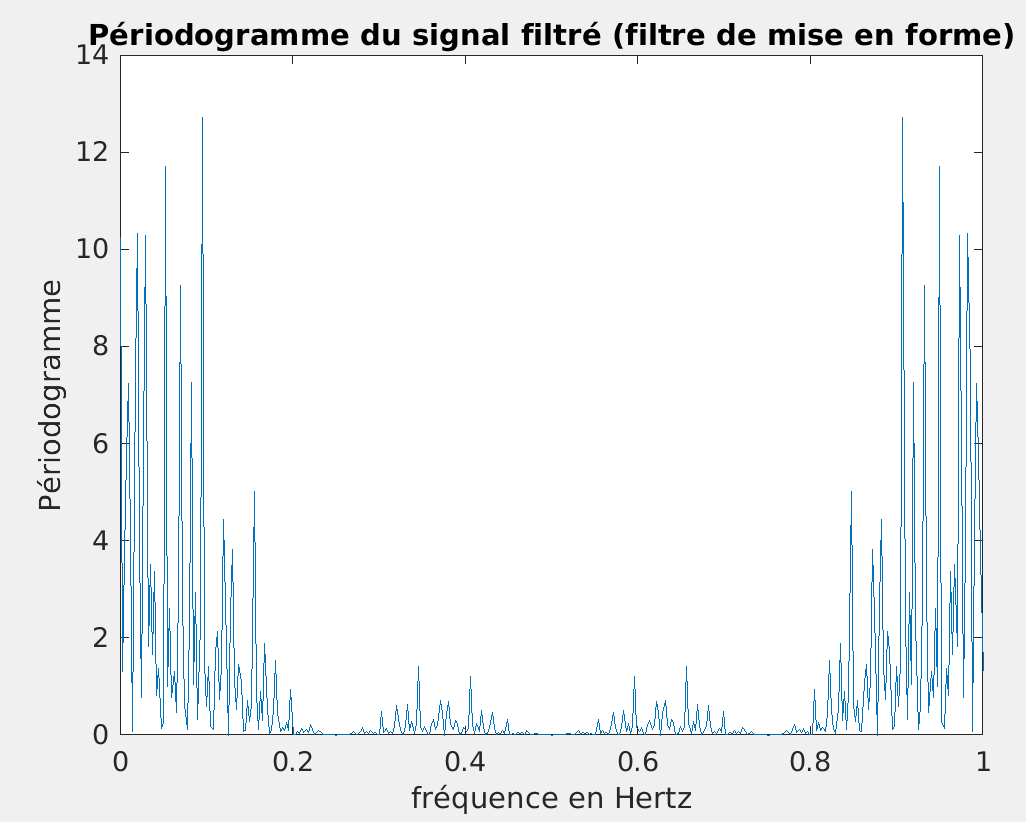
\includegraphics[width=8cm]{C1F42.png}		\caption{DSP du signal transmis (chaîne 1). \label{fig : C1F42}}
		\end{figure}
		
	    D'après l'étude théorique, $ S(f)  = T_s \ sinc^2(\pi f T_s) $ et la bande passante est de $\frac{2}{T_s}$. 
	    
	    Ici, on voit qu'on retrouve les fréquences d'annulation, inférieures à $F_e = 1 Hz$, du sinus cardinal, soit $\frac{1}{T_s} = 0.25 Hz$ et $\frac{2}{T_s} = 0.5 Hz$, ainsi que sa forme. On remarque aussi que la majorité de l'information contenue dans le signal transmis se situe entre $0$ et $0.5 Hz$, en raison de l'amplitude élevée des pics associés. Ainsi, la bande passante est bien de $\frac{2}{T_s}$.
	    \par\leavevmode\par
		
        \item Implantation de la chaine sans bruit :
            \begin{enumerate}
                \item Tracer le signal en sortie du filtre de réception. Ce tracé est-il conforme à ce que vous attendiez (voir étude théorique) ?
                
                \par\leavevmode\par
       			 \setlength\parindent{0.5cm}
        		 La figure \ref{fig : C1F1} représente  le signal en sortie du filtre de réception pour 4000 bits et la figure \ref{fig : C1F12} pour 100 bits.
        
                 \begin{figure}[ht!]
		         \centering
		         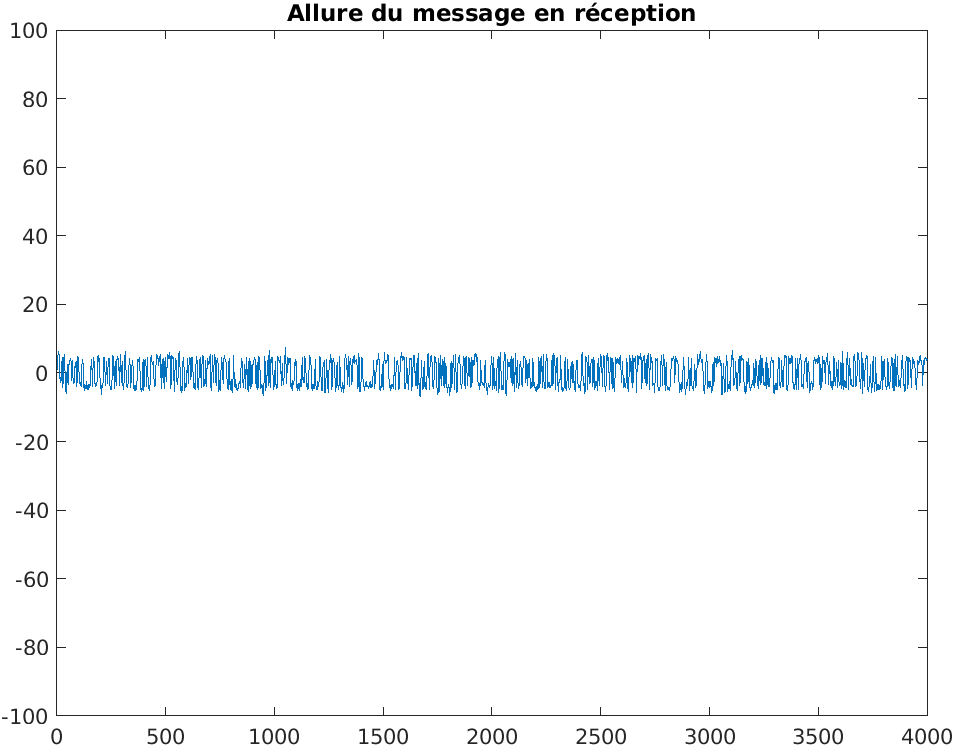
\includegraphics[width=7cm]{C1F1.png}		              			     \caption{Signal en sortie du filtre de réception (4000 bits transmis). \label{fig : C1F1}}
		         \end{figure}
		         
		         \begin{figure}[ht!]
		         \centering
		         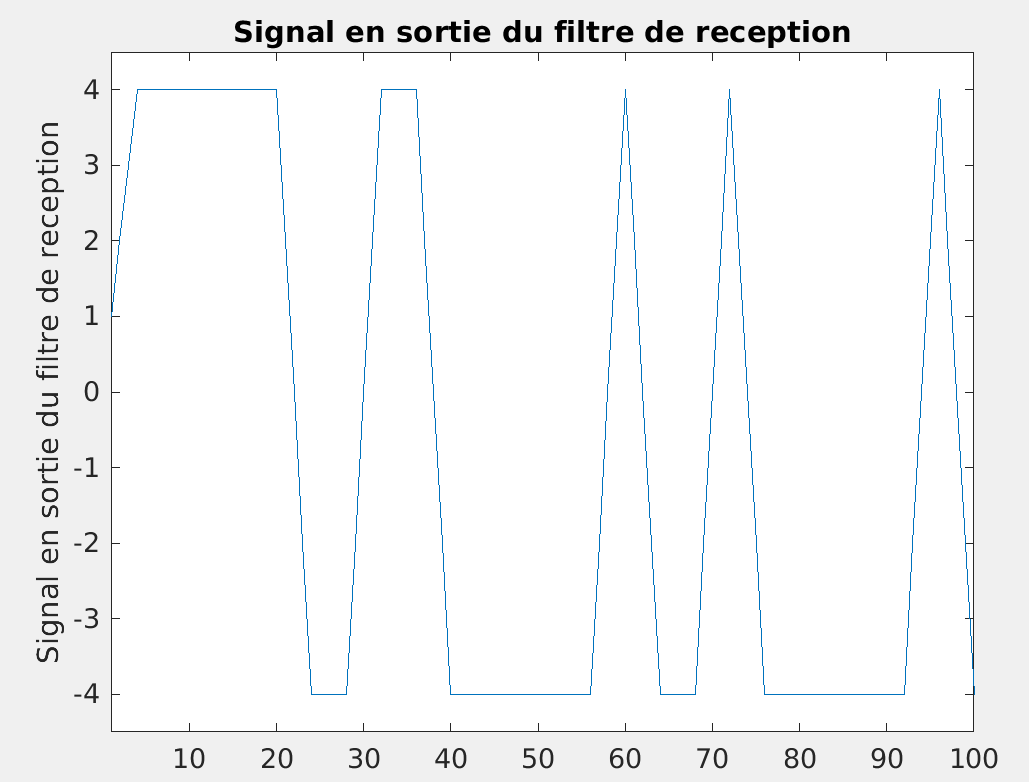
\includegraphics[width=7cm]{C1F12.png}		              			     \caption{Signal en sortie du filtre de réception (100 bits transmis). \label{fig : C1F12}}
		         \end{figure}
				\newpage
				On retrouve bien le résultat théorique car on obtient un signal résultant d'une somme de triangles de largeur $2 T_s$. 
				\par\leavevmode\par

                \item Tracer un diagramme de l'oeil en sortie du filtre de réception afin de déterminer les instants optimaux d'échantilllonnage. Les résultats obtenus sont-ils conformes à la théorie ? Expliquez votre réponse.
                \par\leavevmode\par
       			 \setlength\parindent{0.5cm}
        		 La figure \ref{fig : C1F2} représente  un diagramme de l'oeil en sortie du filtre de réception.
        
                 \begin{figure}[ht!]
		         \centering
		         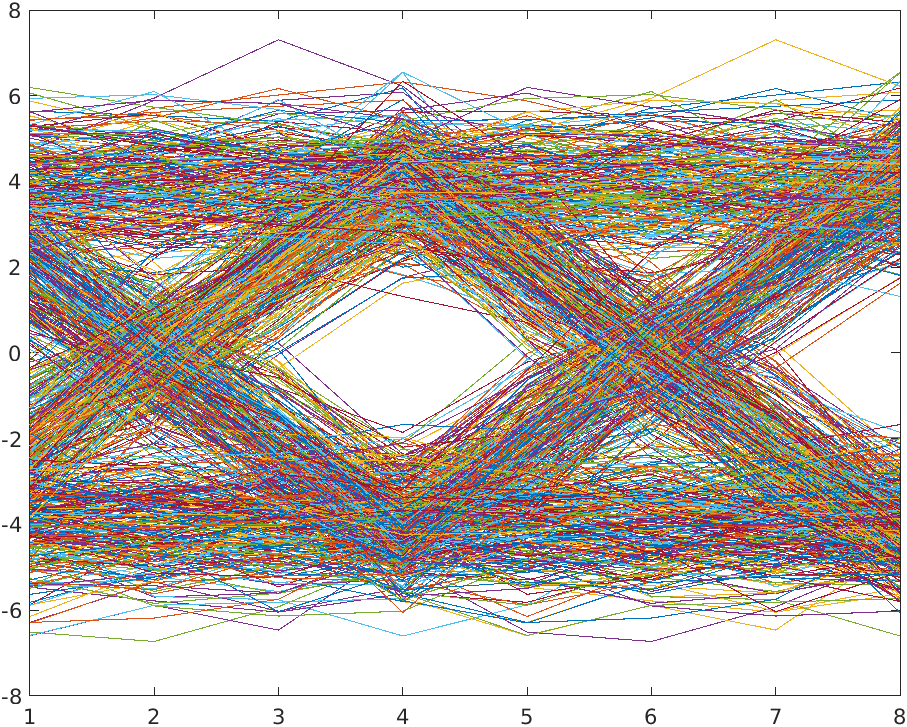
\includegraphics[width=7cm]{C1F2.png}		              			     \caption{Diagramme de l'oeil en sortie du filtre de réception. \label{fig : C1F2}}
		         \end{figure}
		        
				 On remarque ici que $t_0 = T_s$ est l'instant optimal d'échantillonnage, comme c'était le cas dans l'étude théorique. 
				 
				 De plus la forme du diagramme est la même que dans l'étude théorique, la seule différence étant que le nombre de bits transmis  est ici beaucoup plus important que celui pris pour l'étude théorique. 
				\par\leavevmode\par
                \item En utilisant les instants optimaux d'échantillonnage puis un détecteur à seuil, avec seuil optimal, vérifier que le TEB obtenu est bien nul.
                 \par\leavevmode\par
       			 \setlength\parindent{0.5cm}
       			 Avec $t_0 = T_s$ et un seuil à $0$, le TEB est bien nul. 
       		     \par\leavevmode\par	 
            \end{enumerate}
            
        \item Implantation de la chaine avec bruit : rajouter le bruit et tracer le taux d'erreur binaire obtenu en fonction du rapport signal à bruit par bit à l'entrée du récepteur ($E_b/N_0$) en décibels\footnote{Attention les TEBs devront être tracés en échelle log et on fera attention à la précision des mesures réalisées (voir en annexe)}. On prendra des valeurs de $\left(E_b/N_0\right)_{dB}$ allant de $0$ à $6$ dB.
        \par\leavevmode\par
       	\setlength\parindent{0.5cm}
       	La figure \ref{fig : C1F6} représente le TEB obtenu en fonction du rapport signal à bruit par bit à l'entrée du récepteur  ($\left(E_b/N_0\right)_{dB}$). 
        
        \begin{figure}[ht!]
		\centering
		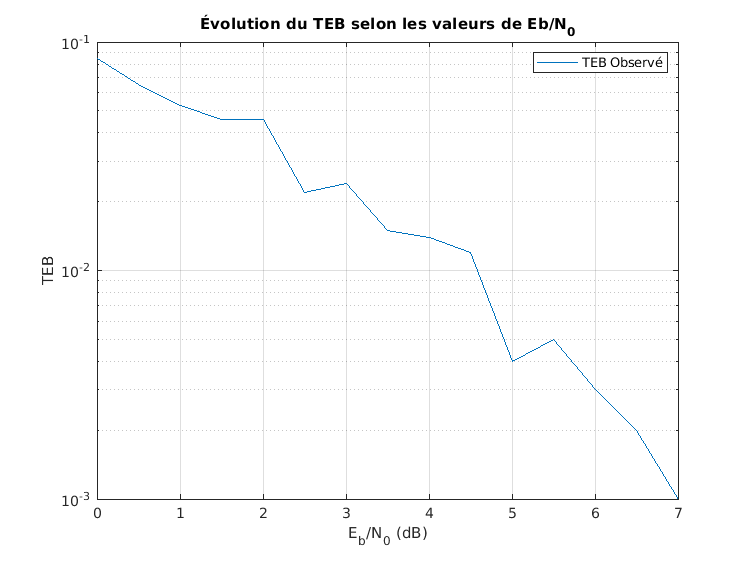
\includegraphics[width=7cm]{C1F6.png}		              	    \caption{TEB obtenu en fonction de $\left(E_b/N_0\right)_{dB}$. \label{fig : C1F6}}
		\end{figure}
		
		\par\leavevmode\par    
        \item Comparer le TEB simulé au TEB théorique de la chaine étudiée (tracé superposés sur une même figure). Ce tracé doit permettre de valider le bon fonctionnement de votre chaine de transmission. La fonction $Q(x)$ peut-être obtenue sou Matlab en utilisant \emph{qfunc.m}.\\
        \par\leavevmode\par
       	
       	La figure \ref{fig : C1F3} représente le TEB simulé et le TEB théorique en fonction du rapport signal à bruit par bit à l'entrée du récepteur  ($\left(E_b/N_0\right)_{dB}$). 
        
        \begin{figure}[ht!]
		\centering
		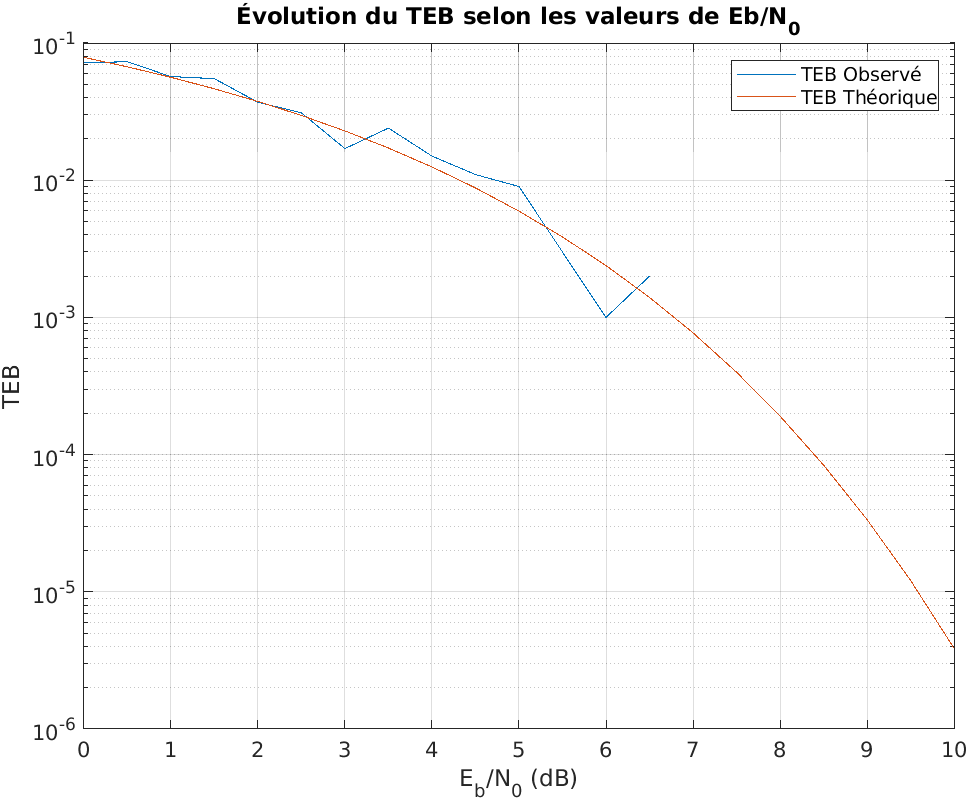
\includegraphics[width=7cm]{C1F3.png}		              	    \caption{TEB simulé et le TEB théorique en fonction de $\left(E_b/N_0\right)_{dB}$. \label{fig : C1F3}}
		\end{figure}
		
		Comme la courbe de TEB simulé tend à suivre celle du TEB théorique, cela permet de valider le bon fonctionnement de notre chaine de transmission.
		
		
    \end{enumerate}

%%%%%%%%%%%%%%%%%%%%%%%%%%%%%%%%%%%%%%%%%%%%%%%%%%%%%%%%%%%%%%%%%%
\section{Deuxième chaine à étudier : impact du choix du filtre de réception}
%%%%%%%%%%%%%%%%%%%%%%%%%%%%%%%%%%%%%%%%%%%%%%%%%%%%%%%%%%%%%%%%%%
On considèrera un mapping binaire à moyenne nulle (symboles $a_k \in \left\{-1,1\right\}$) et les réponses impulsionnelles des filtres de mise en forme et de réception, $h(t$) et $h_r(t)$, données par la figure \ref{rep_imp_ex1_2}. Le résultat du produit de convolution entre $h(t)$ et $h_r(t)$ est donné dans la figure \ref{prod_conv}.

\begin{figure}[ht!]
\centering
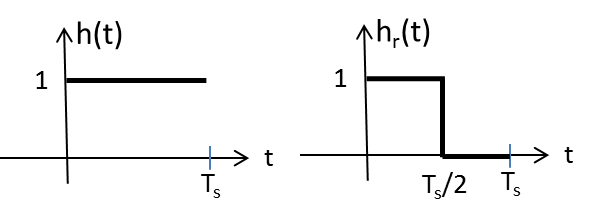
\includegraphics[width=6cm]{figure3.png}
\caption{Réponses impulsionnelles des filtres d'émission et de réception.}
 \label{rep_imp_ex1_2}
\end{figure}

\begin{figure}[ht!]
\centering
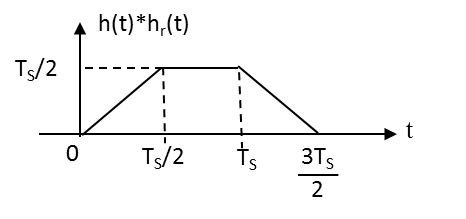
\includegraphics[width=6cm]{figure6.png}
\caption{Produit de convolution entre $h(t)$ et $h_r(t)$.\label{fig : prod_conv}}
\end{figure}

\subsection{Etude théorique}

    \begin{enumerate}
        \item La chaîne de communication peut-elle vérifier le critère de Nyquist ? Justifiez votre réponse.
        \par\leavevmode\par
        \setlength\parindent{0.5cm}
        Le critère de Nyquist en temporel est tel que: 
        \begin{equation*}
        \begin{split}
        \exists t_0 \; \forall l \ne 0 & \; g(t_0 + l T_s) = 0 \\   
        g(t_0) & \ne 0 \\
        \end{split}
        \end{equation*}
        
        D'après la figure \ref{fig : prod_conv}, le critère de Nyquist est réspecté si $t_0 \in \left[\frac{T_s}{2}, T_s\right]$. 
        \par\leavevmode\par
        \item Sans bruit, tracer le signal $z(t)$ en sortie du filtre de réception $h_r(t)$ pour la suite de bits émise suivante : $0110100$. Retrouve-t-on sur ce signal le fait que la chaine de transmission puisse respecter le critère de Nyquist ? Expliquez votre réponse.
        
        \begin{figure}[ht!]
		\centering
		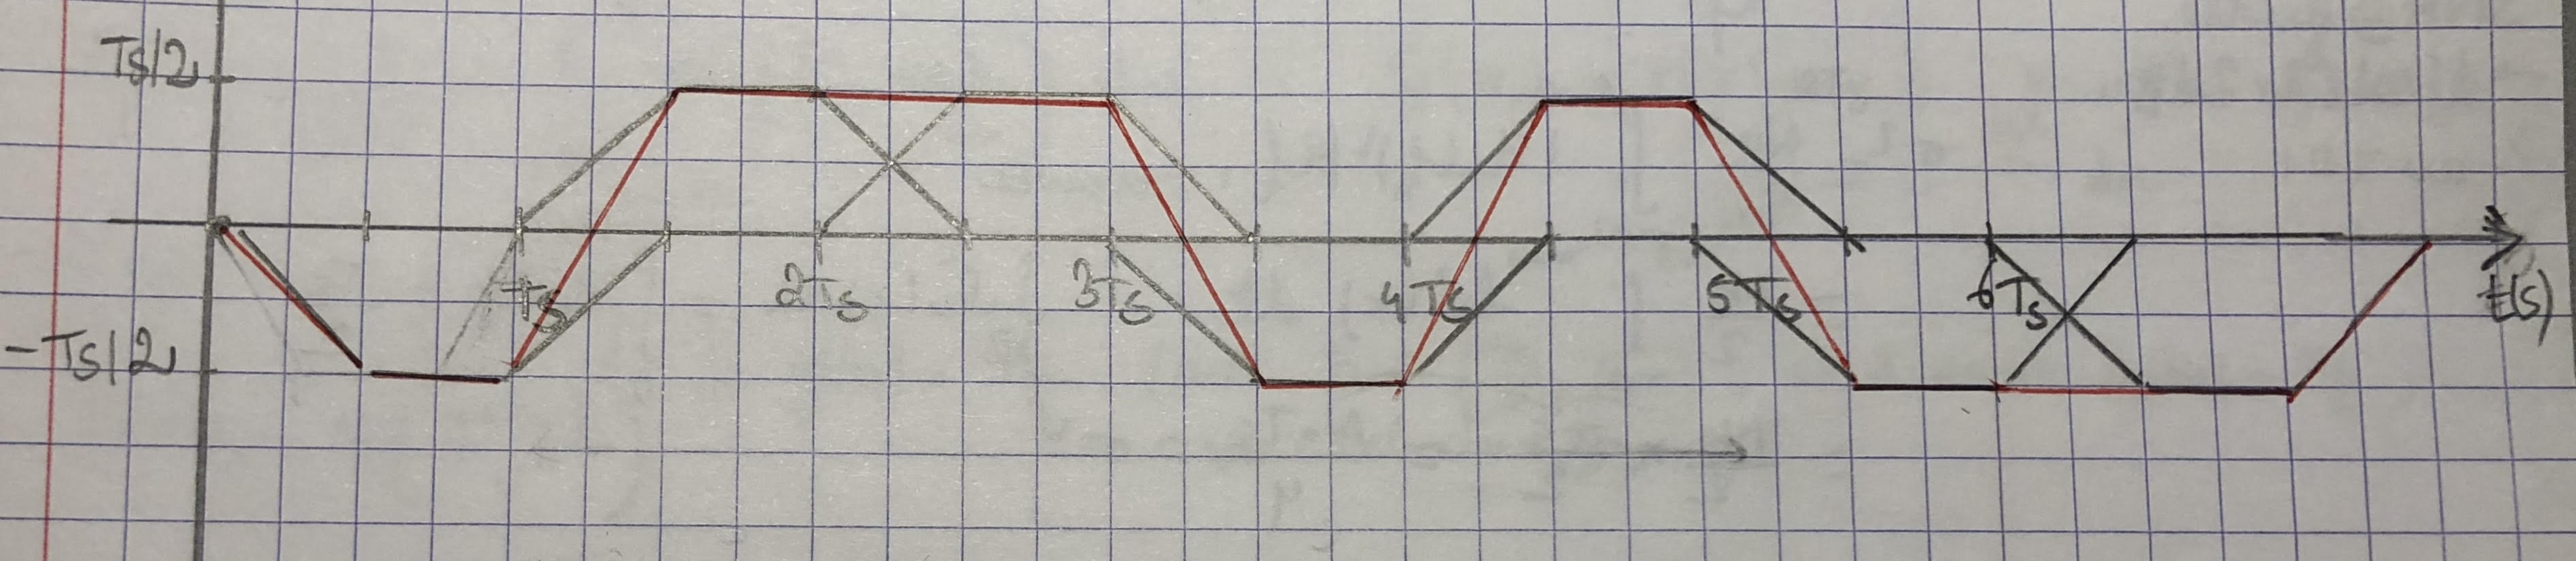
\includegraphics[width=10cm]{C2Q2.jpg}		\caption{Signal $z(t)$ en sortie du filtre de réception $h_r(t)$ pour $0110100$. \label{fig : C2Q2}}
		\end{figure}

        \par\leavevmode\par
        \setlength\parindent{0.5cm}
        Sur la figure \ref{fig : C2Q2}, on voit qu'il n'est pas évident de retrouver à première vue que le critère de Nyquist est respecté. 
        \par\leavevmode\par
        
        \item Toujours sans bruit, tracer le diagramme de l'oeil avec une base de temps de $T_s$. Retrouve-t-on sur le diagramme de l'oeil le fait que la chaine de transmission puisse respecter le critère de Nyquist ? Justifiez votre réponse.
        
        \begin{figure}[ht!]
		\centering
		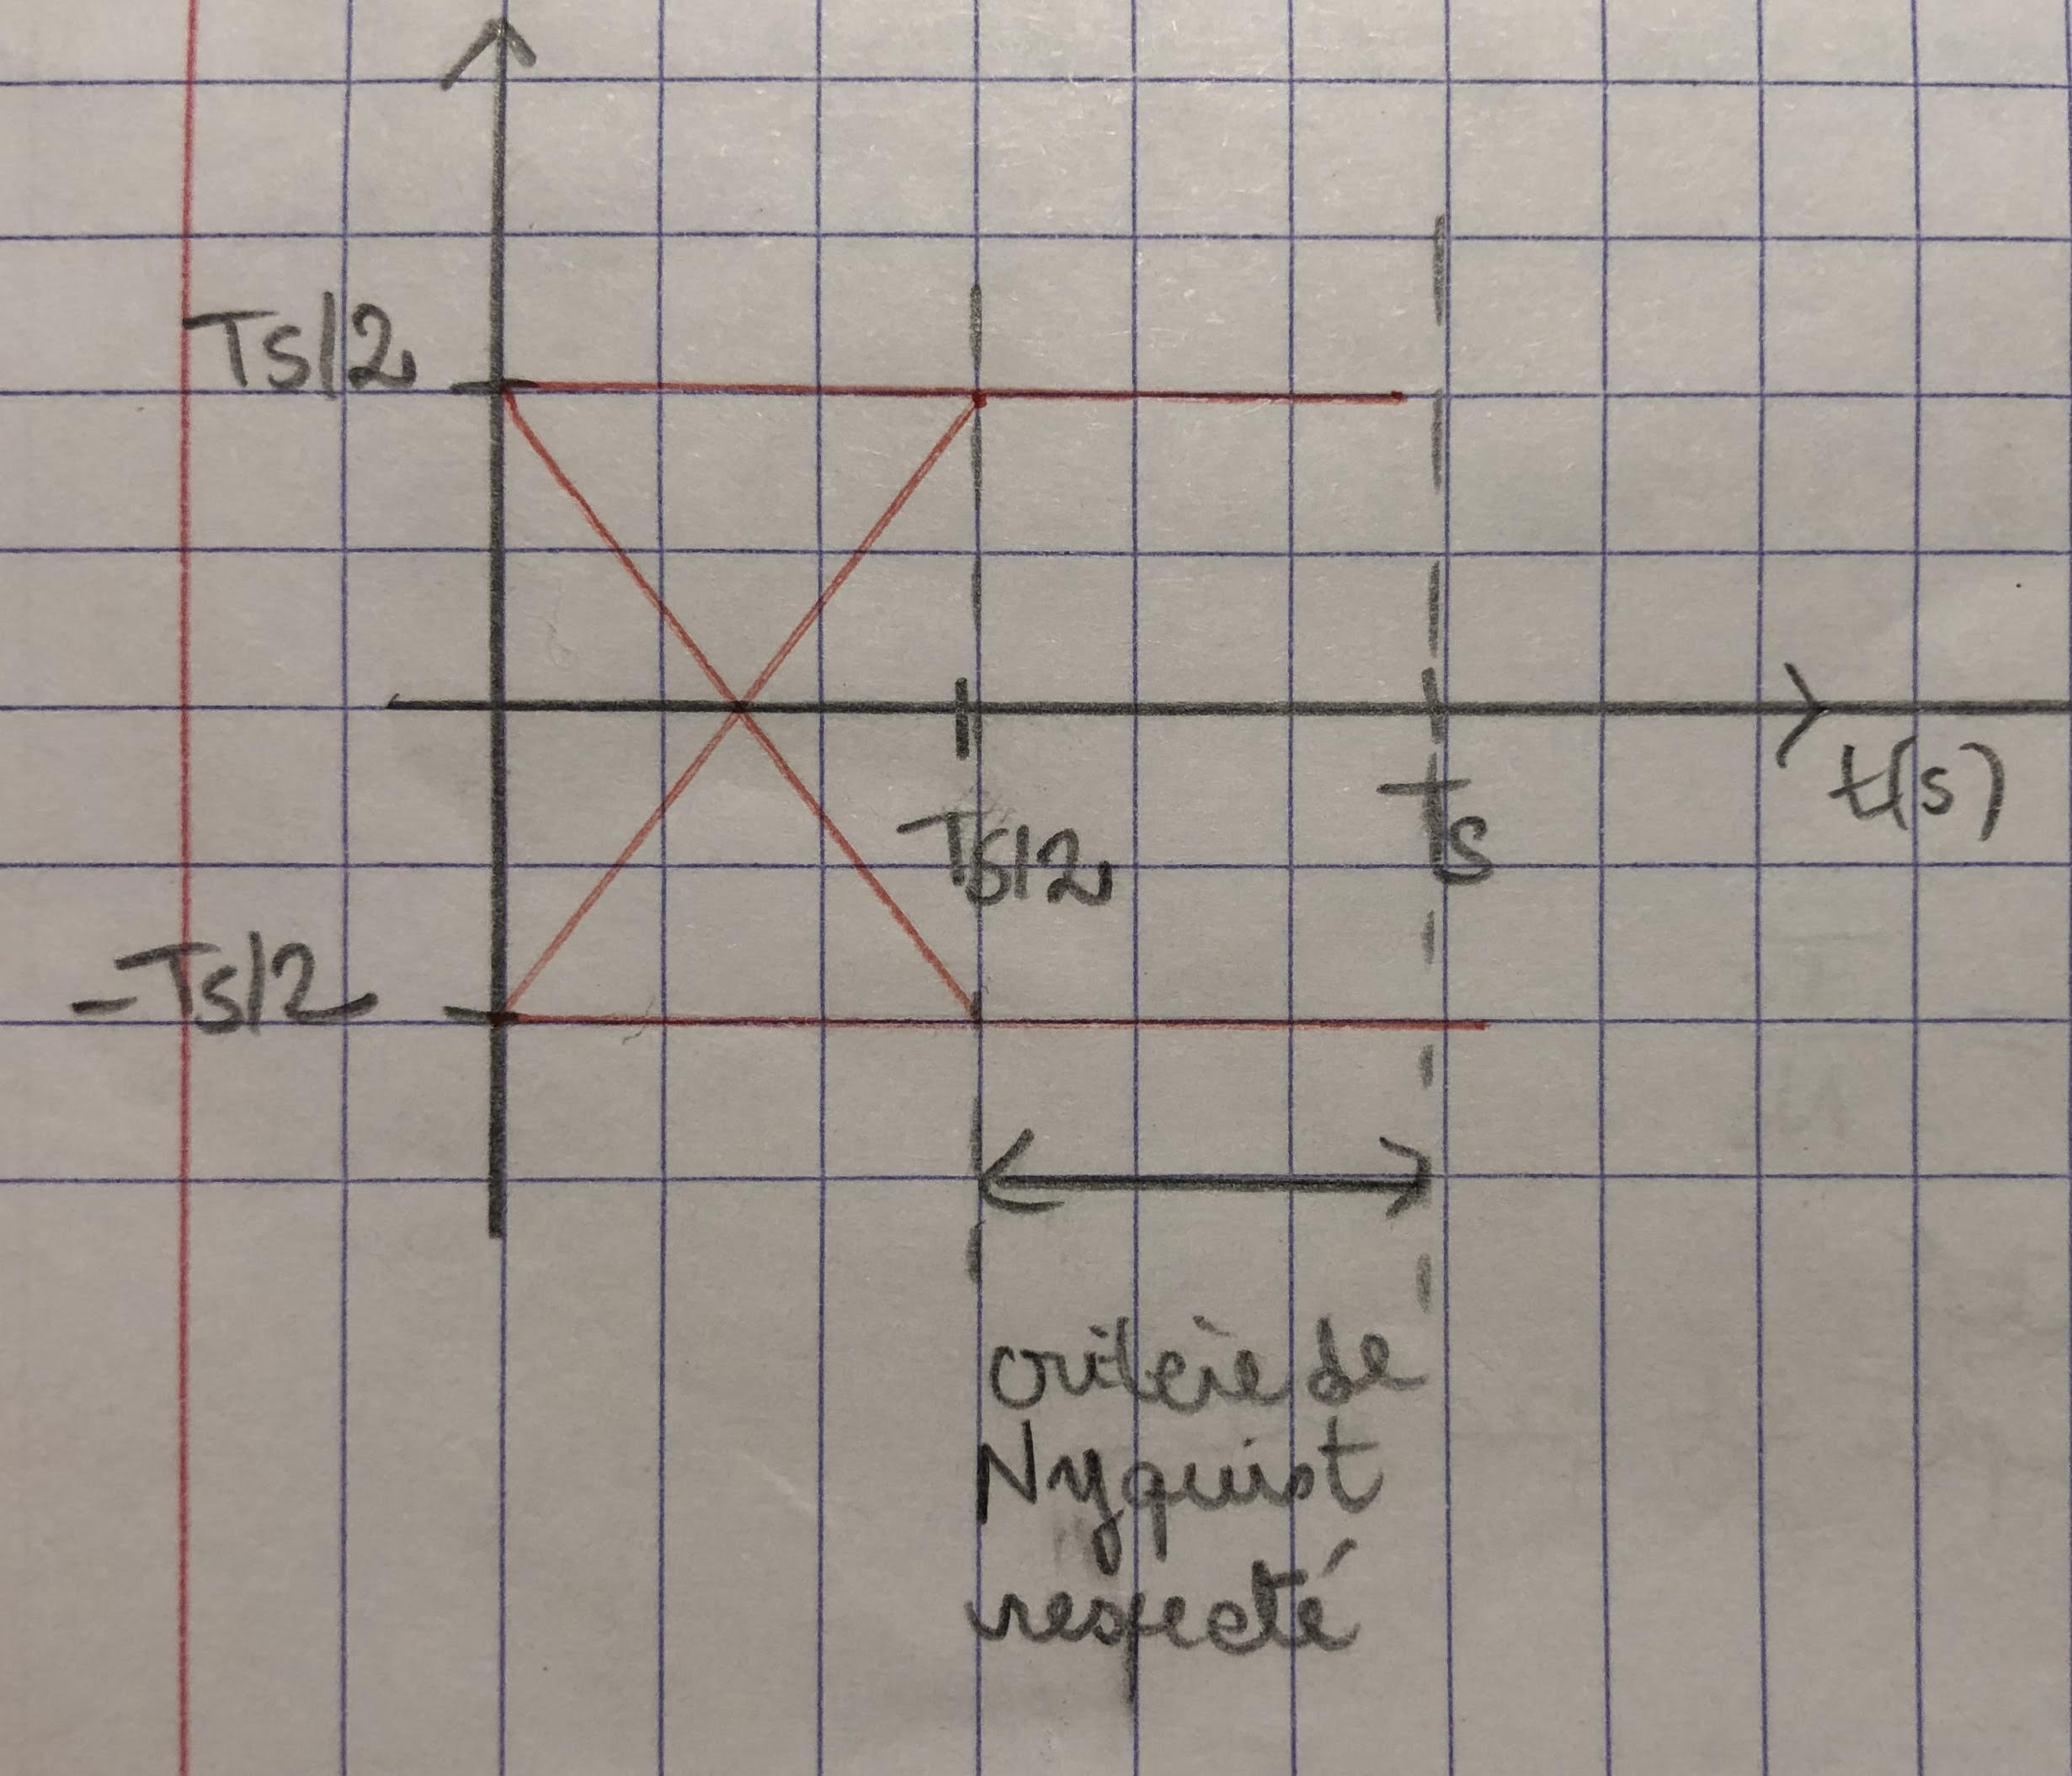
\includegraphics[width=5cm]{C2Q3.jpg}		\caption{Diagramme de l'oeil. \label{fig : C2Q3}}
		\end{figure}

        \par\leavevmode\par
        \setlength\parindent{0.5cm}
        Sur la figure \ref{fig : C2Q3}, on voit ici que le critère de Nyquist est réspecté pour:
        $$\boxed{t_0 \in \left[\frac{T_s}{2}, T_s\right]}$$
         \par\leavevmode\par
        \item En supposant que l'on échantillonne aux instants optimaux (sans ISI), calculer le rapport signal sur bruit aux instants d'échantillonnage (on admettra que la puissance du bruit échantillonné et filtré est identique à celle du bruit filtré et on calculera donc cette puissance en sortie du filtre de réception). Comparer le rapport signal sur bruit obtenu ici avec celui obtenu dans la chaine de référence. Que peut-on supposer sur la comparaison des TEBs des deux chaines de transmission ?
        
        \begin{equation*}
        \begin{split}
        SNR & = \frac{P_s}{\sigma^2} \\        
        z_m &= a_m g(t_0)\\
        z_m & = a_m \frac{T_s}{2}\\
        P_s & = \mathbb{E}\left(\left(a_m \frac{T_s}{2}\right)^2\right) \\
        P_s & = \mathbb{E}\left(\frac{T_s^2}{4}\right) \\
        P_s & = \frac{T_s^2}{4}
        \end{split}
        \end{equation*}
         
        D'après la définition de la puissance du bruit:
        
        \begin{equation*}
        \begin{split}
        P_{\omega} &= \int_\mathbb{R}S_{\omega}(f) \ \mathrm{d}f \\
        \end{split}
        \end{equation*}
        
        D'après la formule de Wiener-Lee:
        
        \begin{equation*}
        \begin{split}
        P_{\omega} = \int_{\mathbb{R}}|H_r(f)|^2 \frac{N_0}{2} \ \mathrm{d}f \\
        \end{split}
        \end{equation*}
        
        D'après notammant l'égalité de Parseval, on en déduit:
        \begin{equation*}
        \begin{split}
        \sigma^2 &= \frac{N_0}{2} \frac{T_s}{2}  \\
        \sigma &= \frac{\sqrt{N_0 T_s}}{2}
        \end{split}
        \end{equation*}
        
        Donc: 
        \begin{equation*}
        \begin{split}
        \boxed{SNR = \frac{T_s}{N_0}}  \\
        \end{split}
        \end{equation*}
        
        \begin{equation*}
        \begin{split}
        SNR = \frac{1}{2} \ SNR_{chaîneref} \\
        SNR < SNR_{chaîneref} \\
        \end{split}
        \end{equation*}
        
        Donc on peut supposer que le TEB de cette chaîne sera plus important que celui de la chaîne de référence. 
        \par\leavevmode\par
        
        \item On choisira d'utiliser un détecteur à seuil. Déterminer le seuil optimal à utiliser en expliquant votre choix.
        
        \par\leavevmode\par
        \setlength\parindent{0.5cm}
        On choisit 0 comme seuil, car on dispose d'une gaussienne centrée sur $T_s$ et d'une autre gaussienne centrée sur $- T_s$, en ce qui concerne $\mathbb{P}(z_m)$.
        \par\leavevmode\par
        \item En supposant que l'on échantillonne aux instants optimaux et que l'on utilise le seuil optimal de décision, donner le taux d'erreur binaire de la transmission en fonction de $T_s$ et $\sigma$, $\sigma^2$ représentant la puissance du bruit en sortie du filtre de réception $h_r(t)$.
        
        \par\leavevmode\par
        \begin{equation*}
        \begin{split}
        TEB & = \mathbb{P}(\hat{a}_m \ne a_m) \\
        & = \frac{1}{2} \mathbb{P}\left(\hat{a}_m = + 1 \ | \ a_m = -1\right) + \frac{1}{2} \mathbb{P}\left(\hat{a}_m = - 1 \ | \ a_m = +1\right) \\
        & = \mathbb{P}\left(\hat{a}_m = + 1 \ | \ a_m = -1\right) \\
        & = \mathbb{P}\left(z_m \geq 0 \ | \ z_m = -\frac{T_s}{2} + \omega_m\right) \\
        & = \mathbb{P}\left(\frac{\omega_m}{\sigma} \geq \frac{T_s}{2 \sigma}\right) \\
        \end{split}
        \end{equation*}
        
        Comme $\frac{\omega_m}{\sigma}$ suit une loi centrée réduite: 
        $$\boxed{TEB = Q\left(\frac{T_s}{2 \sigma}\right)}$$
        
        \item Calculer la puissance du bruit en sortie du filtre de réception $\sigma^2$ en fonction de $N_0$ et de $T_s$.
        \par\leavevmode\par
        D'après la question $4$: 
        $$\boxed{\sigma^2 = \frac{N_0 T_s}{4}}$$
        \par\leavevmode\par
        
        \item Calculer l'énergie des symboles à l'entrée du récepteur, $E_s$, en fonction de $T_s$.
        \par\leavevmode\par
        Au symbole $a_k$, est associé, à l'entrée du récepteur, le signal $a_k h(t-kT_s)$.
        \begin{equation*}
        \begin{split}
        E_s &= \int_{\mathbb{R}} \left(a_k h(t-kT_s)\right)^2 \ \mathrm{d}t \\
        & = \int_{\mathbb{R}} \left(h^2(t)\right) \ \mathrm{d}t \\
        & = T_s \\        
        \end{split}
        \end{equation*}
        \par\leavevmode\par
        \item Déduire des questions précédentes l'expression du taux d'erreur binaire en fonction de $E_b/N_0$ pour la chaine étudiée.
        \par\leavevmode\par
        D'après la question $6$:
        $$ TEB = Q\left(\frac{T_s}{2 \sigma}\right) $$
        
        Or:
        \begin{equation*}
        \begin{split}
        \frac{T_s}{2 \sigma} &= \frac{T_s}{\sqrt{N_0 T_s}} \\
        & = \sqrt{\frac{T_s}{N_0}} \\
        & = \sqrt{\frac{E_s}{N_0}} \\
        \end{split}
        \end{equation*}
        
        Donc:
        $$\boxed{TEB = Q\left(\sqrt{\frac{E_s}{N_0}}\right)} $$
    \end{enumerate}

\subsection{Implantation sous Matlab}
    \begin{enumerate}
        \item Implantation de la chaine sans bruit (le signal à transmettre sera généré en tronquant la bande occupée à une fréquence maximale égale à $\frac{4}{T_s}$)
            \begin{enumerate}
                \item Tracer le signal en sortie du filtre de réception. Ce tracé est-il conforme à ce que vous attendiez (voir étude théorique) ?
                
                 \par\leavevmode\par
                 \setlength\parindent{0.5cm}
                 La figure \ref{fig : C2F1} représente  le signal en sortie du filtre de réception pour 4000 bits et la figure \ref{fig : C2F12} pour 100 bits.
        
                 \begin{figure}[ht!]
		         \centering
		         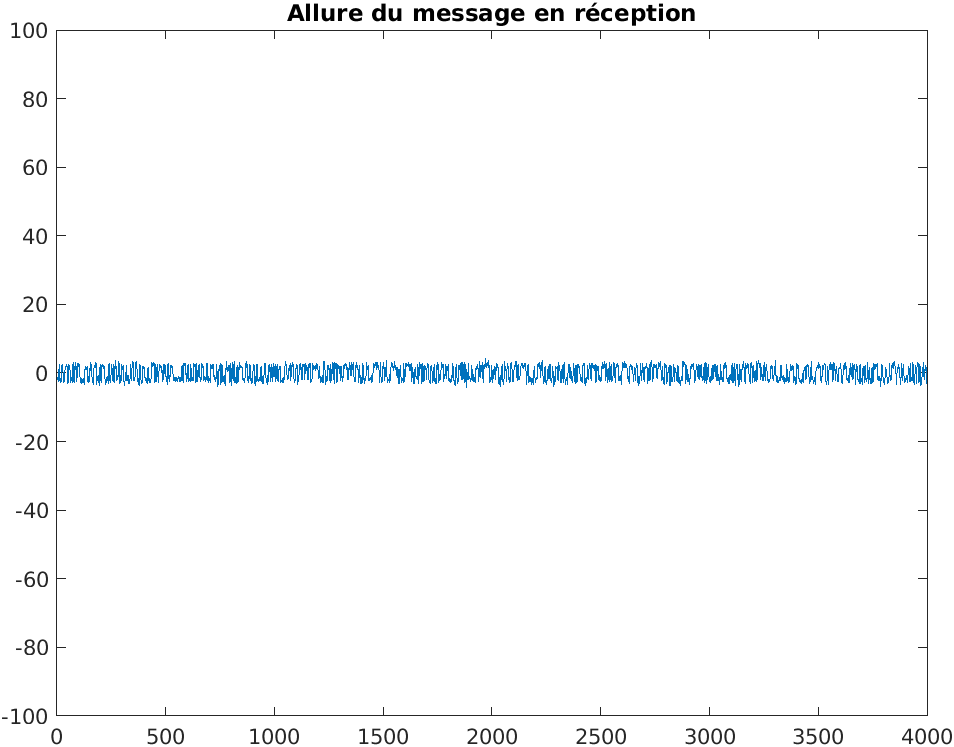
\includegraphics[width=5cm]{C2F1.png}		              			     \caption{Signal en sortie du filtre de réception (4000 bits transmis). \label{fig : C2F1}}
		         \end{figure}
		         
		         \begin{figure}[ht!]
		         \centering
		         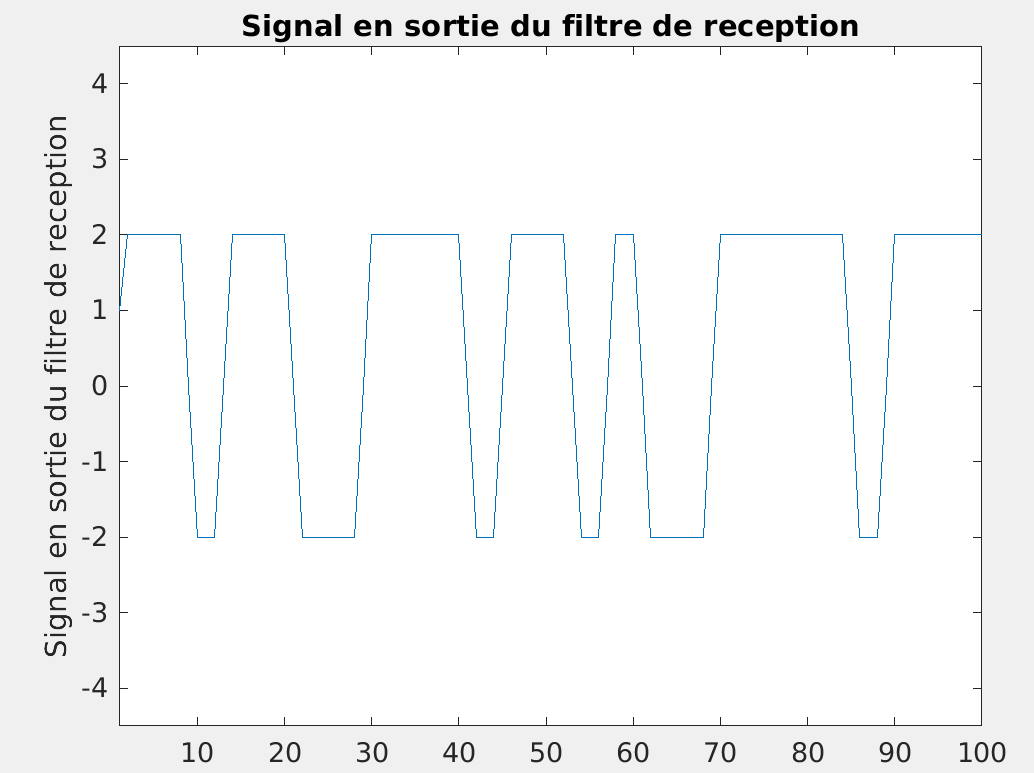
\includegraphics[width=7cm]{C2F12.png}		              			     \caption{Signal en sortie du filtre de réception (100 bits transmis). \label{fig : C2F12}}
		         \end{figure}
				 \newpage
				 On retrouve bien le résultat théorique car on obtient un signal résultant d'une somme de trapèzes de largeur $\frac{3 T_s}{2}$ et d'amplitude $\frac{T_s}{2}$.
				 
				 Lorsque l'on a deux signaux dont le symbole est le même, la longeur sur laquelle le signal est constant de $\frac{T_s}{2}$ est de $1.5 T_s = 6s$, ce qui est bien le cas aussi dans l'étude théorique.
				 
                Lorsque deux signaux dont le symbole n'est pas le même se suivent, la plus petite distance entre les deux morceaux de signaux constants est de $2.5 T_s = 2s$.
                
				Ce raisonnement se poursuit pour une continuité plus importante de signaux associés au même symbole. 
				 \par\leavevmode\par
                \item Tracer un diagramme de l'oeil en sortie du filtre de réception afin de déterminer les instants optimaux d'échantilllonnage. Les résultats obtenus sont-ils conformes à la théorie ? Expliquez votre réponse.
                \par\leavevmode\par
       			 \setlength\parindent{0.5cm}
        		 La figure \ref{fig : C2F1} représente  un diagramme de l'oeil en sortie du filtre de réception.
        
                 \begin{figure}[ht!]
		         \centering
		         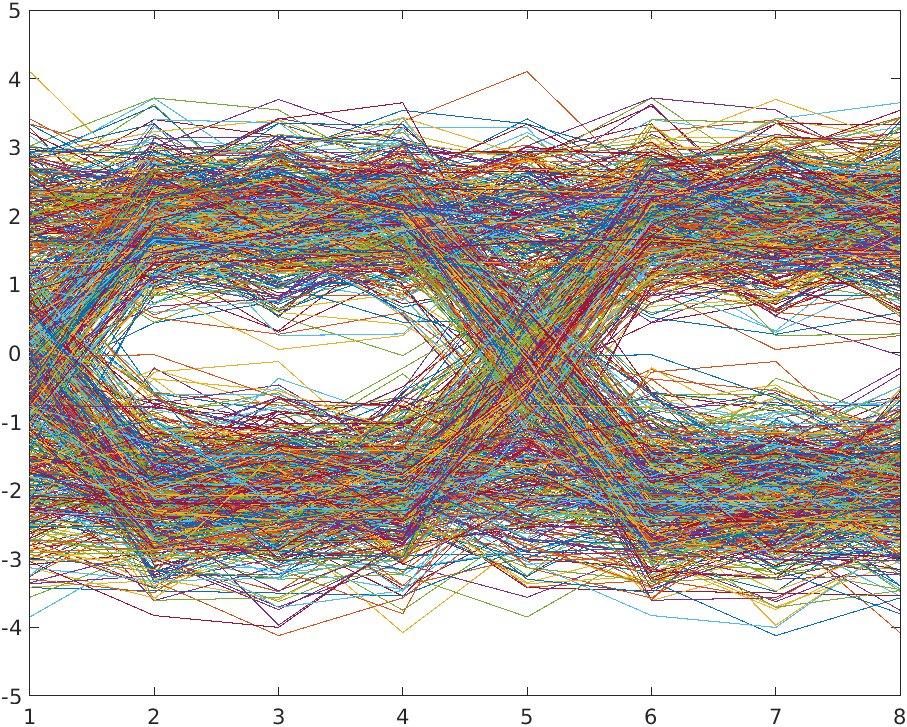
\includegraphics[width=7cm]{C2F2.png}		              			     \caption{Diagramme de l'oeil en sortie du filtre de réception (chaîne 2). \label{fig : C2F2}}
		         \end{figure}
		        
		        \newpage
				 On remarque ici que tout $t_0 \in \left[\frac{T_s}{2}, T_s\right] = \left[2, 4\right]$ peut être pris comme instant optimal d'échantillonnage, comme c'était le cas dans l'étude théorique. 
				 
				 De plus la forme du diagramme est la même que dans l'étude théorique, la seule différence étant que le nombre de bits transmis  est ici beaucoup plus important que celui pris pour l'étude théorique. 
                \item En utilisant les instants optimaux d'échantillonnage puis un détecteur à seuil, avec seuil optimal, vérifier que le TEB obtenu est bien nul.
                \par\leavevmode\par
       			 \setlength\parindent{0.5cm}
       			 Avec $t_0 = T_s$ et un seuil à $0$, le TEB est bien nul. 
       		     \par\leavevmode\par
            \end{enumerate}
        \item Implantation de la chaine avec bruit : rajouter le bruit et tracer le taux d'erreur binaire obtenu en fonction du rapport signal à bruit par bit à l'entrée du récepteur ($E_b/N_0$) en décibels. On prendra des valeurs de $\left(E_b/N_0\right)_{dB}$ allant de $0$ à $6$ dB.
        \par\leavevmode\par
       	\setlength\parindent{0.5cm}
       	La figure \ref{fig : C2F6} représente le TEB obtenu en fonction du rapport signal à bruit par bit à l'entrée du récepteur  ($\left(E_b/N_0\right)_{dB}$). 
        
        \begin{figure}[ht!]
		\centering
		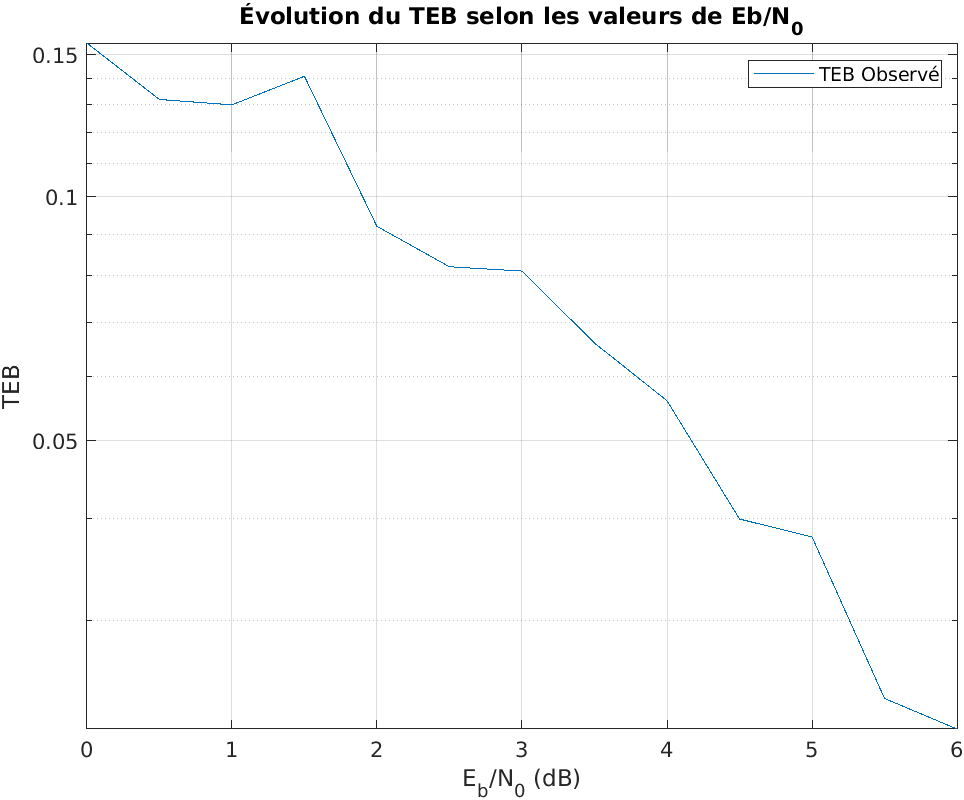
\includegraphics[width=7cm]{C2F6.png}		              	    \caption{TEB obtenu en fonction de $\left(E_b/N_0\right)_{dB}$ (chaîne 2). \label{fig : C2F6}}
		\end{figure}
		
		\par\leavevmode\par
        \item Comparer le TEB simulé au TEB théorique de la chaine étudiée (tracé superposés sur une même figure). Ce tracé doit permettre de valider le bon fonctionnement de votre chaine de transmission.
        \par\leavevmode\par
       	
       	La figure \ref{fig : C2F3} représente le TEB simulé et le TEB théorique en fonction du rapport signal à bruit par bit à l'entrée du récepteur  ($\left(E_b/N_0\right)_{dB}$). 
        
        \begin{figure}[ht!]
		\centering
		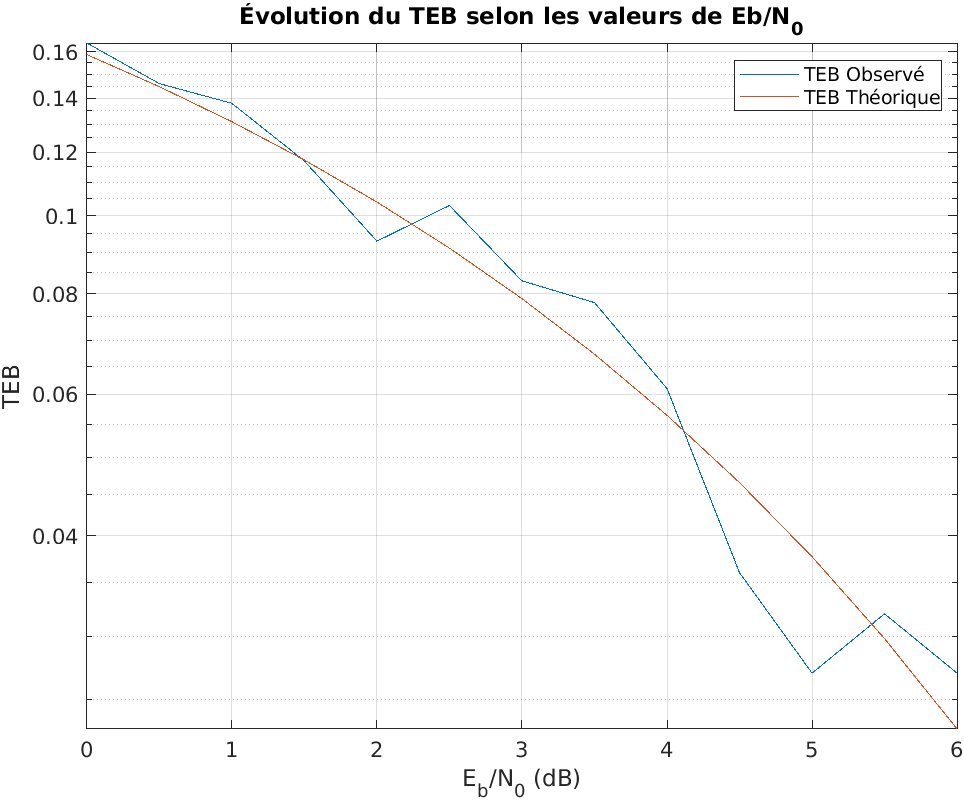
\includegraphics[width=7cm]{C2F3.png}		              	    \caption{TEB simulé et le TEB théorique en fonction de $\left(E_b/N_0\right)_{dB}$. \label{fig : C2F3}}
		\end{figure}
		\newpage
		Comme la courbe de TEB simulé tend à suivre celle du TEB théorique, cela permet de valider le bon fonctionnement de notre chaine de transmission.
		\par\leavevmode\par
        \item Comparer le TEB obtenu par simulation pour la chaine de transmission étudiée au TEB obtenu par simulation (ou au TEB théorique) de la chaine de référence (comparaison en termes d'efficacité en puissance). La similitude ou différence obtenue devra être expliquée. La chaine éventuellement la plus efficace en puissance devra être identifiée, en expliquant pourquoi.
        \par\leavevmode\par
       	\setlength\parindent{0.5cm}
       	La figure \ref{fig : C2F5} représente le TEB obtenu par simulation pour la chaine de transmission étudiée et le TEB obtenu par simulation de la chaine de référence  des signaux transmis.
        
        \begin{figure}[ht!]
		\centering
		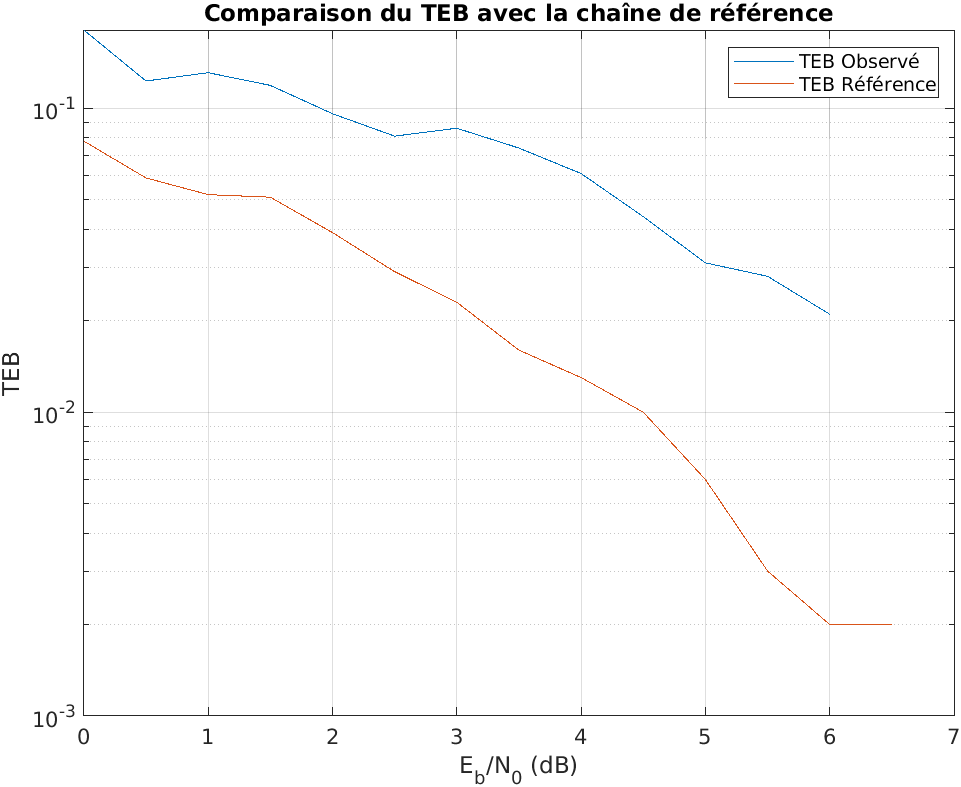
\includegraphics[width=9cm]{C2F5.png}		              	    \caption{TEB simulé de la chaîne 2 et TEB simulé de la chaîne de référence en fonction de $\left(E_b/N_0\right)_{dB}$. \label{fig : C2F5}}
		\end{figure}

		On remarque que, pour un même TEB, dans la chaîne de référence, il y a besoin d'une plus faible valeur de $E_s$ pour obtenir ce TEB, par à rapport à la chaine étudiée. 
		
		C'était le cas ausi dans l'étude théorique.
		 
		Donc, théorie et pratique s'accordent pour dire que la chaîne de référence est la plus efficace en puissance.

		
		
		\par\leavevmode\par
        \item Comparer l'efficacité spectrale de la chaine étudiée avec celle de la chaine de référence (en traçant, par exemple, les DSPs des signaux transmis dans les deux cas pour un même débit binaire). La similitude ou différence obtenue devra être expliquée. La chaine éventuellement la plus efficace spectralement devra être identifiée, en expliquant pourquoi.
        \par\leavevmode\par
       	\setlength\parindent{0.5cm}
       	La figure \ref{fig : C2F52} représente les DSPs des signaux transmis, pour la chaîne étudiée et la chaîne de référence. 
       	
        
        \begin{figure}[ht!]
		\centering
		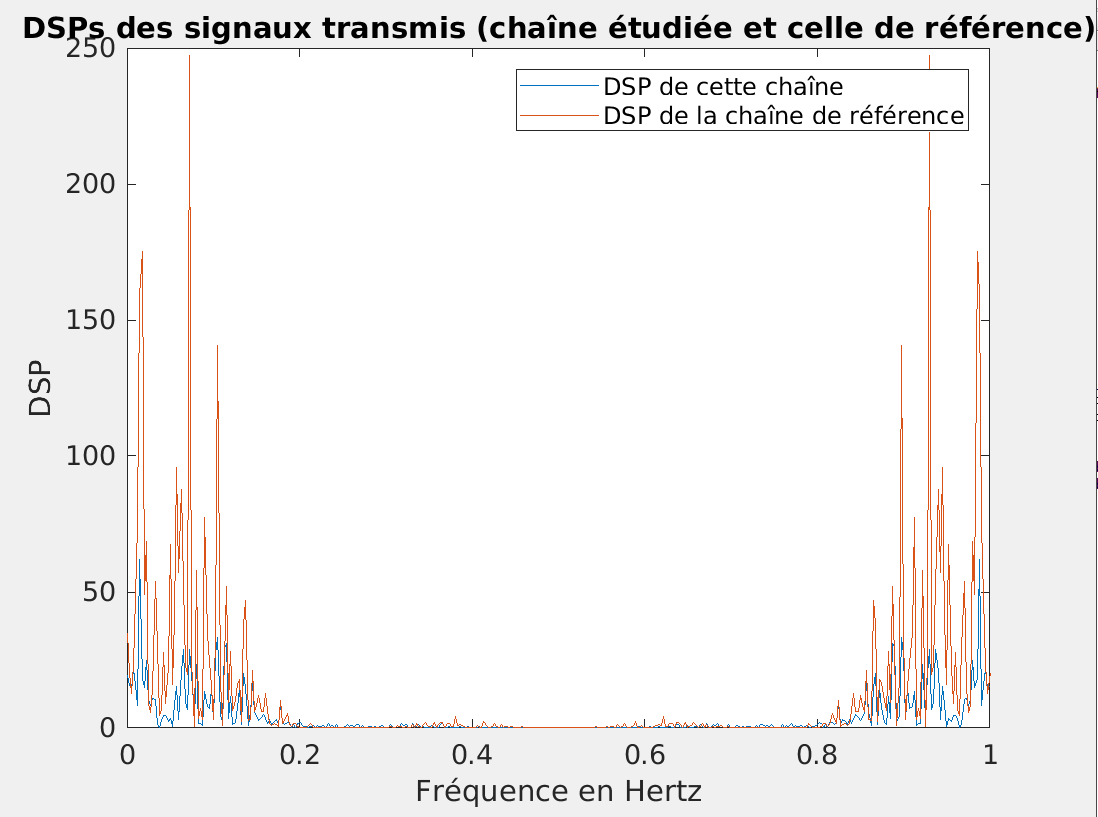
\includegraphics[width=9cm]{C2F52.png}		              	    \caption{DSPs de la chaîne 2 et de la chaîne de référence. \label{fig : C2F52}}
		\end{figure}
		
		La chaîne la plus efficace spectralement est celle dont la courbe de la DSP est telle qu'elle montre qu'un maximum de l'information est contenu dans une faible bande de fréquence. 
		
		Ici, elles ont la même bande passante.
		
		Donc, elles ont la même efficacité spectrale. 
		
    \end{enumerate}

%%%%%%%%%%%%%%%%%%%%%%%%%%%%%%%%%%%%%%%%%%%%%%%%%%%%%%%%%%%%%%%%%%
\section{Troisième chaine à étudier : impact du choix du filtre de mise en forme et d'un canal de propagation à bande limitée}
%%%%%%%%%%%%%%%%%%%%%%%%%%%%%%%%%%%%%%%%%%%%%%%%%%%%%%%%%%%%%%%%%%
On considèrera un mapping binaire à moyenne nulle (symboles $a_k \in \left\{-1,1\right\}$) et des réponses impulsionnelles des filtres de mise en forme et de réception, $h(t$) et $h_r(t)$, en racine de cosinus surélevé de même roll off $\alpha=0.5$. Le résultat du produit de convolution entre $h(t)$ et $h_r(t)$ est donc un cosinus surélevé de roll off $0.5$.

\subsection{Etude théorique}

    \begin{enumerate}
        \item La chaîne de communication peut-elle vérifier le critère de Nyquist ? Justifiez votre réponse.
        \par\leavevmode\par
        \setlength\parindent{0.5cm}
        Le critère de Nyquist dans le domaine fréquentiel est: 
        \begin{equation*}
        \begin{split}
        \sum\limits_{k \in \mathbb{K}}{G^{t_0}\left(f-\frac{k}{T_s} \right)} =  \text{cste}\\
        \text{avec} \ G^{t_0}(f) = \mathrm{TF}\left(\frac{g\left(t_0 + t\right)}{g\left(t_0 \right)}\right) \\
        \end{split}
        \end{equation*}
        
        On considère la figure \ref{fig : C3Q1}:
        
        \begin{figure}[ht!]
        \centering
        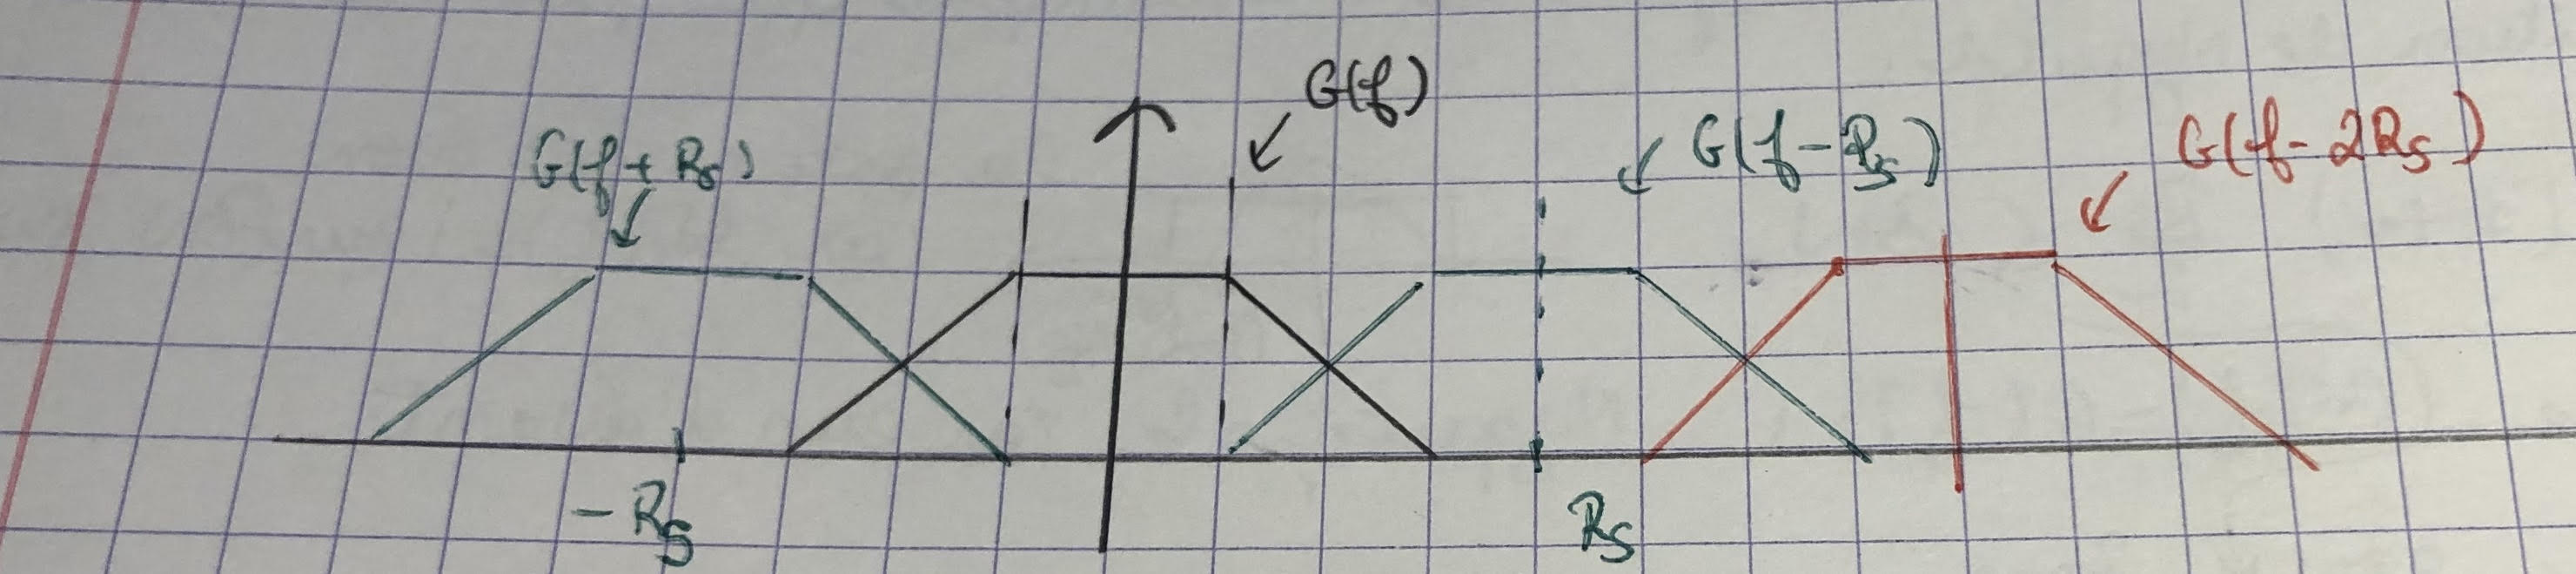
\includegraphics[width = 9cm]{C3Q1.jpg}
        \caption{Tracé utile pour la vérification du critère de Nyquist en fréquentiel. \label{fig : C3Q1}}
        \end{figure}
        
        Pour $f \in \left[0, R_s \right[$, $G(f) + G(f-R_s) = \text{cste}$.
        
        Donc, cette chaîne peut vérifier le critère de Nyquist. 
        \par\leavevmode\par
        \item La chaîne de communication vérifie t-elle le critère de filtrage adapté ? Justifiez votre réponse.
        \par\leavevmode\par
        \setlength\parindent{0.5cm}
        Un filtre adapté est tel que: $h_r(t) = \lambda \ h^*(t_0-t)$. 
        
        En prenant 	$\lambda = 1$ et $t_0 = 0$, on a bien un filtre de réception adapté. 
       \par\leavevmode\par
        \item Donner (sans le calculer) le taux d'erreur binaire théorique de la transmission, en justifiant votre choix de formule.
        \par\leavevmode\par
        \setlength\parindent{0.5cm}
        Comme  la chaîne satisfait le critère de Nyquist: $TEB = Q\left(\frac{g(t_0}{\sigma}\right)$. 
        
        Comme la chaîne vérifie le critère de filtrage adapté, le $TEB$ est minimal et est égal à: $$ \boxed{TEB = Q\left(\sqrt{\frac{2 E_b}{N_0}}\right)}$$
        
        \par\leavevmode\par
        
        \item A quelle condition, sur le rythme symbole $R_s$, pourrait-on transmettre le signal généré par le modulateur proposé dans un canal de transmission idéal de bande $BW=1500$ Hz, tout en continuant de respecter le critère de Nyquist ?
        \par\leavevmode\par
        \setlength\parindent{0.5cm}
        La condition, sur $R_s$ à respecter pour transmettre le signal généré par le modulateur proposé dans un canal de transmission idéal de bande $BW=1500$ Hz, tout en continuant de respecter le critère de Nyquist, se déduit de l'inégalité suivante:
        $$ (1 + \alpha) \frac{R_s}{2} \leq \text{BW} $$
        
        Et le critère de Nyquist reste respecté car:
        \begin{equation*}
        \begin{split}
        G^\prime(f)  = H(f) \ H_c(f) \ H_r(f) \\
        G^\prime(f)  = H(f) \ H_r(f) \ H_c(f)  \\
        \end{split}
        \end{equation*}
        
        \setlength\parindent{3cm}
        et avec la condition contenue dans l'inégalité,
        $G^\prime(f)  = G(f) \mathrm{x} 1 $
        
        \setlength\parindent{0.5cm}
        Donc:
        $$\boxed{R_s \leq \frac{2 \text{BW}}{1 + \alpha}}$$
        \par\leavevmode\par
        \item Afin d'implanter la chaine de transmission en numérique, quelle est la fréquence d'échantillonnage minimum à utiliser ? En déduire le facteur de suréchantillonnage minimal à utiliser.
        \par\leavevmode\par
        \setlength\parindent{0.5cm}
        On doit vérifier: 
        $$ F_e \geq 2 F_{max}$$
        $$ F_e \geq (1 + \alpha) R_s = 1.5 R_s $$
        
        Pour avoir un nombre entier d'échantillons: $F_e\geq 2 R_s$
        
        Donc la fréquence d'échantillonnage minimum à utiliser est $\boxed{F_e = 2 R_s}$, et le facteur de suréchantillonnage minimum à utiliser est $\boxed{N_s = 2}$. 
        
           
    \end{enumerate}

\subsection{Implantation sous Matlab}

    \begin{enumerate}
        \item On utilisera les paramètres suivants : fréquence d'échantillonnage $F_e=12000$ Hz, rythme symbole $R_s=3000$ symboles par seconde, roll off du filtre de mise en forme et du filtre de réception $\alpha=0.5$.
        \item Implantation de la chaine sans bruit :
            \begin{enumerate}
                \item Le facteur de suréchantillonnage utilisé ici permet-il de respecter la condition d'échantillonnage de Shannon ? Justifiez votre réponse.
                
                \par\leavevmode\par
                \setlength\parindent{0.5cm}
                On a: $ F_e = N_s R_s = 12000$ Hz et $R_s = 3000$ Hz. 
                
                Donc: $N_s = 4 < (N_s)_{min}=2$
                
                Donc, le facteur de suréchantillonnage permet de respecter le crirère de Shannon.
                \par\leavevmode\par
                
                
                \item Tracer le signal en sortie du filtre de réception. Ce tracé est-il conforme à ce que vous attendiez (voir étude théorique) ? Expliquez votre réponse.
                \par\leavevmode\par
                \setlength\parindent{0.5cm}
                La figure \ref{fig : C3F1} représente  le signal en sortie du filtre de réception pour 4000 bits et la figure \ref{fig : C3F12} pour 100 bits.
        
                 \begin{figure}[ht!]
		         \centering
		         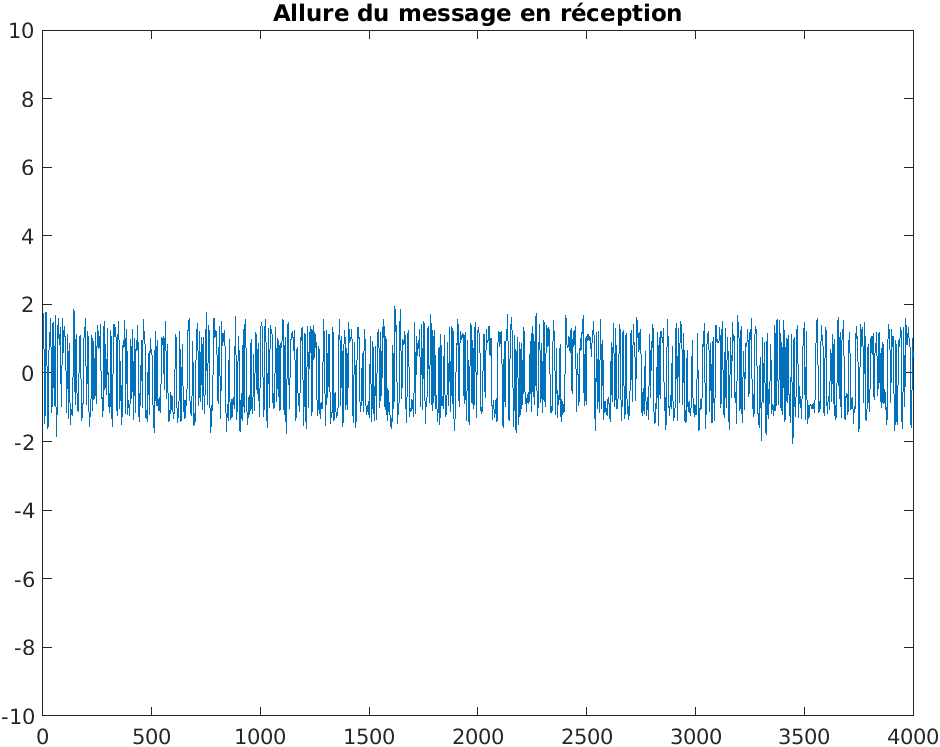
\includegraphics[width=5cm]{C3F1.png}		              			     \caption{Signal en sortie du filtre de réception (4000 bits transmis)(chaîne 3). \label{fig : C3F1}}
		         \end{figure}
		         
		         \begin{figure}[ht!]
		         \centering
		         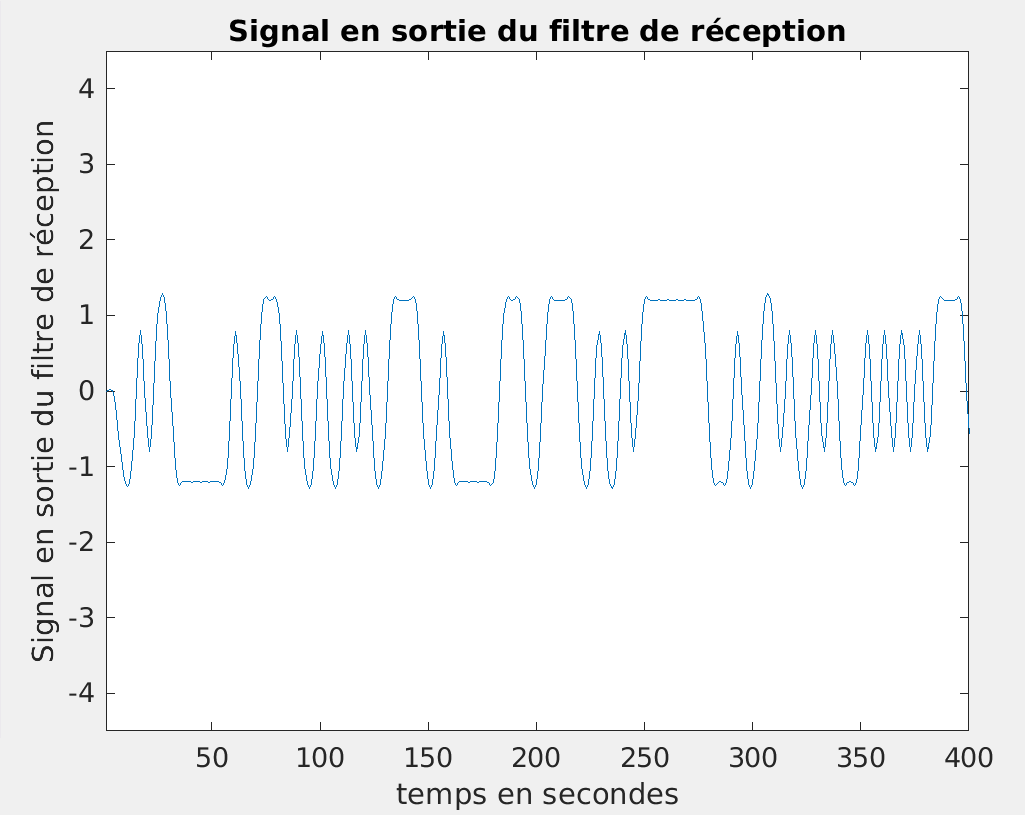
\includegraphics[width=7cm]{C3F12.png}		              			     \caption{Signal en sortie du filtre de réception (100 bits transmis)(chaîne 3). \label{fig : C3F12}}
		         \end{figure}
				 \newpage
				Ce tracé est conforme à l'étude théorique réalisée en amont. On observe bien la superposition de cosinus surélevés pondérés par 1 ou -1 et distants de Ts.  
                
                \par\leavevmode\par
                \item Tracer un diagramme de l'oeil en sortie du filtre de réception afin de déterminer les instants optimaux d'échantilllonnage. Les résultats obtenus sont-ils conformes à la théorie ? Justifiez votre réponse.
                \par\leavevmode\par
       			 \setlength\parindent{0.5cm}
        		 La figure \ref{fig : C3F2} représente  un diagramme de l'oeil en sortie du filtre de réception.
        
                 \begin{figure}[ht!]
		         \centering
		         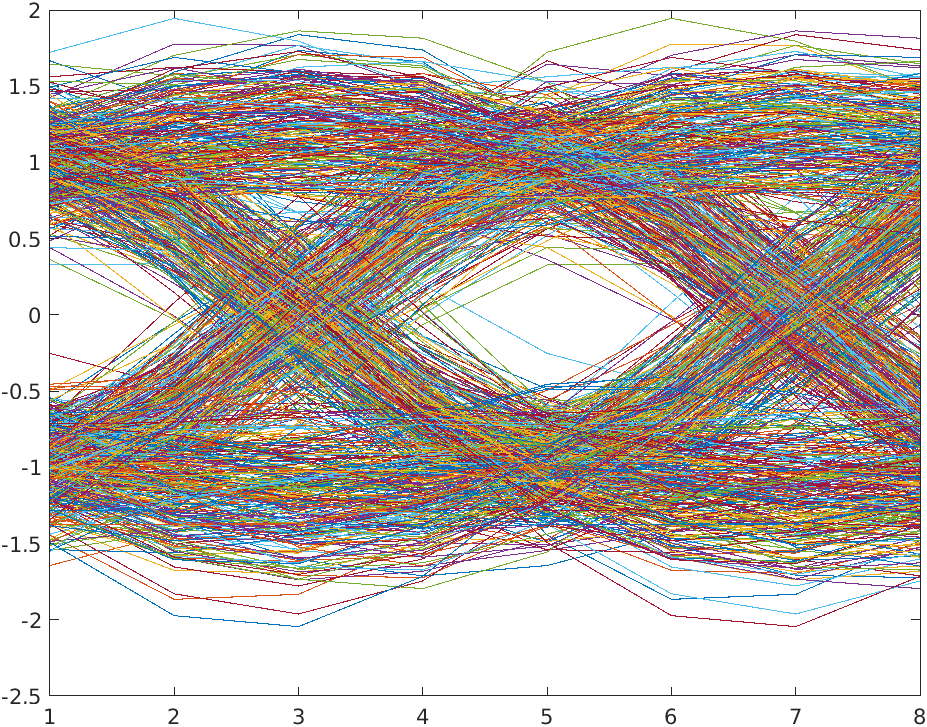
\includegraphics[width=7cm]{C3F2.png}		              			     \caption{Diagramme de l'oeil en sortie du filtre de réception (chaîne 3). \label{fig : C3F2}}
		         \end{figure}
		         
		         On prend $t_0 = 0$ comme instant d'échantillonnage optimal. 
		          
		         \par\leavevmode\par
                \item En utilisant les instants optimaux d'échantillonnage puis un détecteur à seuil, avec seuil optimal, vérifier que le TEB obtenu est bien nul. Attention ici aux retards introduits par les filtres de la chaine de transmission qui excèdent la durée d'un symbole.
                \par\leavevmode\par
       			 \setlength\parindent{0.5cm}
       			 Avec $t_0 = 0$ et un seuil à $0$, le TEB est bien nul. 
       			 
       			 Remarque sur le retard induit par le filtrage: Comme on a un retard introduit par les filtres, il faut supprimer ce retard lors du calcul du TEB. On choisit alors de calculer le TEB sur moins de bits que ceux envoyés. Le retard est lié à de combien il faut décaler la réponse impulsionnelle pour la rendre causale.
Ici le cosinus surélevé est centré en 0.
Donc pour le rendre causal, il faut le translater d'au minimum $\frac{longueur_{filtre}}{2}$.
       			 
       		     \par\leavevmode\par
            \end{enumerate}
        \item Implantation de la chaine avec bruit : rajouter le bruit et tracer le taux d'erreur binaire (TEB) obtenu en fonction du rapport signal à bruit par bit à l'entrée du récepteur ($E_b/N_0$) en décibels. On prendra des valeurs de $\left(E_b/N_0\right)_{dB}$ allant de $0$ à $6$ dB.
        \par\leavevmode\par
       	\setlength\parindent{0.5cm}
       	La figure \ref{fig : C3F6} représente le TEB obtenu en fonction du rapport signal à bruit par bit à l'entrée du récepteur  ($\left(E_b/N_0\right)_{dB}$). 
        
        \begin{figure}[ht!]
		\centering
		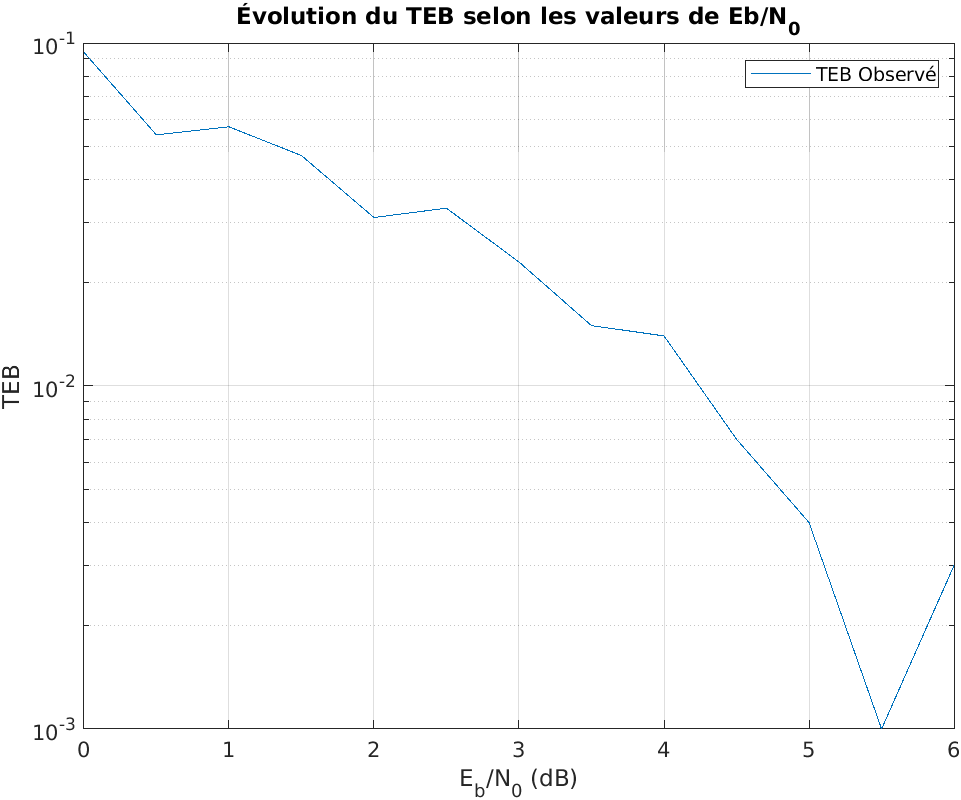
\includegraphics[width=7cm]{C3F6.png}		              	    \caption{TEB obtenu en fonction de $\left(E_b/N_0\right)_{dB}$ (chaîne 3). \label{fig : C3F6}}
		\end{figure}
		
		\par\leavevmode\par
        \item Comparer le TEB simulé au TEB théorique de la chaine étudiée (tracé superposés sur une même figure). Ce tracé doit permettre de valider le bon fonctionnement de votre chaine de transmission.
        \par\leavevmode\par
       	\setlength\parindent{0.5cm}
       	La figure \ref{fig : C3F3} représente le TEB simulé et le TEB théorique en fonction du rapport signal à bruit par bit à l'entrée du récepteur  ($\left(E_b/N_0\right)_{dB}$). 
        
        \begin{figure}[ht!]
		\centering
		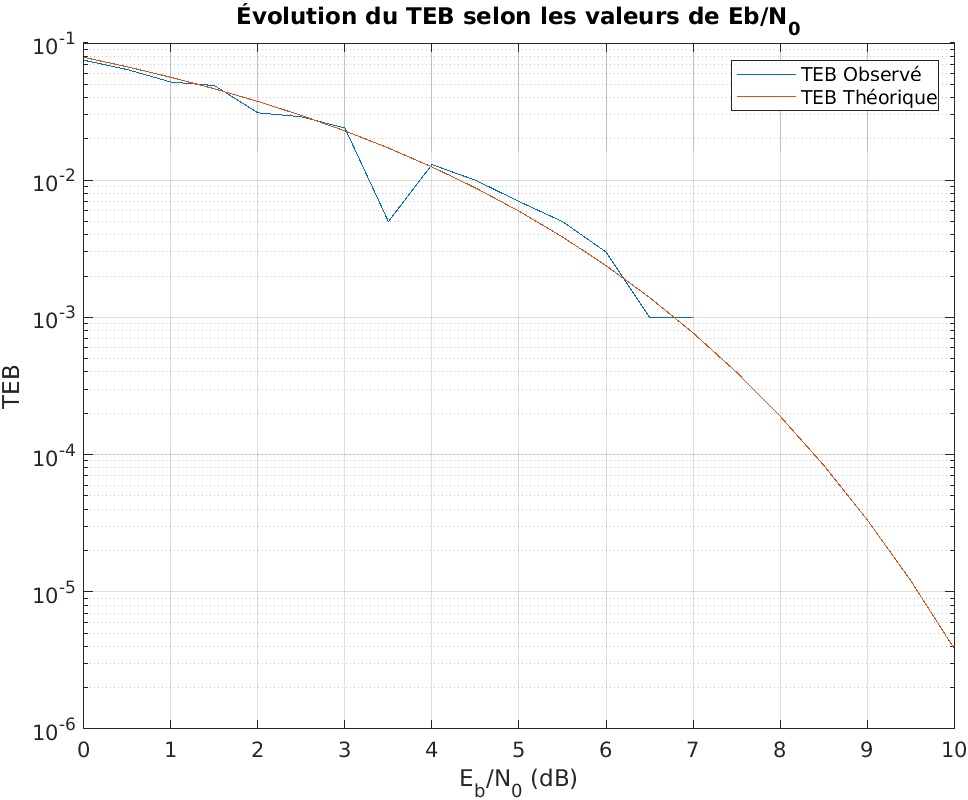
\includegraphics[width=7cm]{C3F3.png}		              	    \caption{TEB simulé et le TEB théorique en fonction de $\left(E_b/N_0\right)_{dB}$ (chaîne 3). \label{fig : C2F3}}
		\end{figure}
		\newpage
		Comme la courbe de TEB simulé tend à suivre celle du TEB théorique, cela permet de valider le bon fonctionnement de notre chaine de transmission.
		\par\leavevmode\par
        
        \item Comparer le TEB obtenu par simulation pour la chaine de transmission étudiée au TEB obtenu par simulation (ou au TEB théorique) de la chaine de référence (comparaison en termes d'efficacité en puissance). La similitude ou différence obtenue devra être expliquée. La chaine éventuellement la plus efficace en puissance devra être identifiée, en expliquant pourquoi.
        \par\leavevmode\par
       	\setlength\parindent{0.5cm}
       	La figure \ref{fig : C3F5} représente le TEB obtenu par simulation pour la chaine de transmission étudiée et le TEB obtenu par simulation de la chaine de référence  des signaux transmis.  
        
        \begin{figure}[ht!]
		\centering
		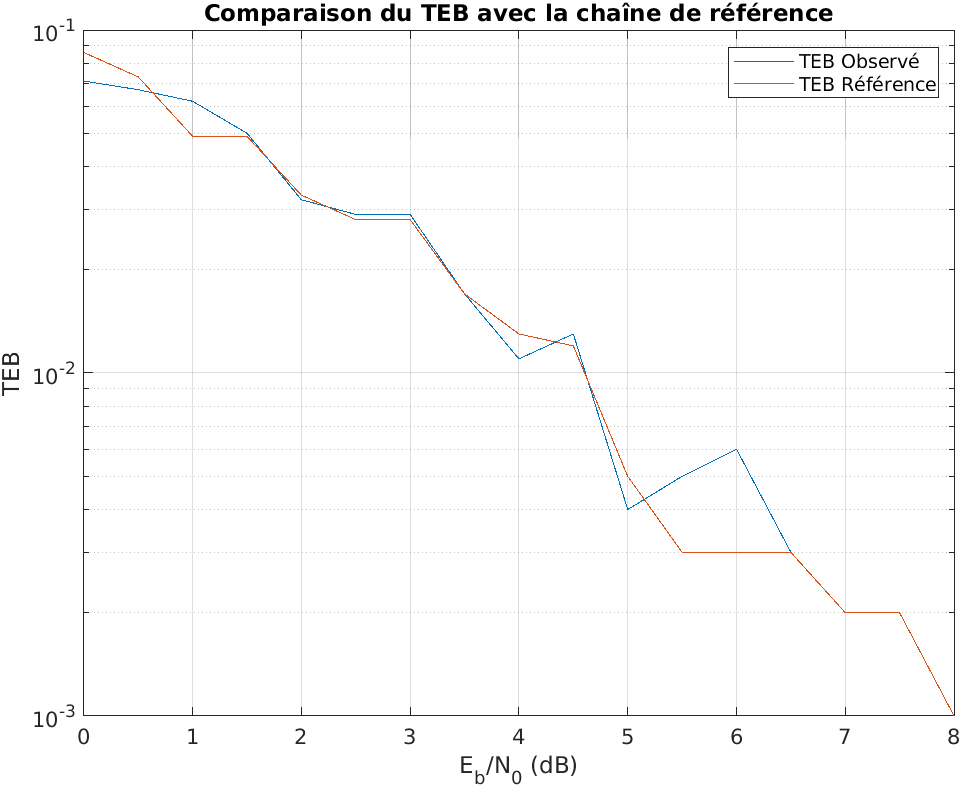
\includegraphics[width=7cm]{C3F5.png}		              	    \caption{TEB simulé de la chaîne 3 et TEB simulé de la chaîne de référence en fonction de $\left(E_b/N_0\right)_{dB}$. \label{fig : C3F5}}
		\end{figure}
		
		On remarque que les deux courbes sont presque confondues. Cela est en accord avec la partie théorique car l'expression de leur TEB est la même. 
		\par\leavevmode\par
        \item Comparer l'efficacité spectrale de la chaine étudiée avec celle de la chaine de référence (en traçant les DSPs des signaux transmis dans les deux cas pour un même débit binaire). La similitude ou différence obtenue devra être expliquée. La chaine éventuellement la plus efficace spectralement devra être identifiée, en expliquant pourquoi.
        \par\leavevmode\par
       	\setlength\parindent{0.5cm}
       	La figure \ref{fig : C3F52} représente les DSPs des signaux transmis, pour la chaîne étudiée et la chaîne de référence. 
       	
        
        \begin{figure}[ht!]
		\centering
		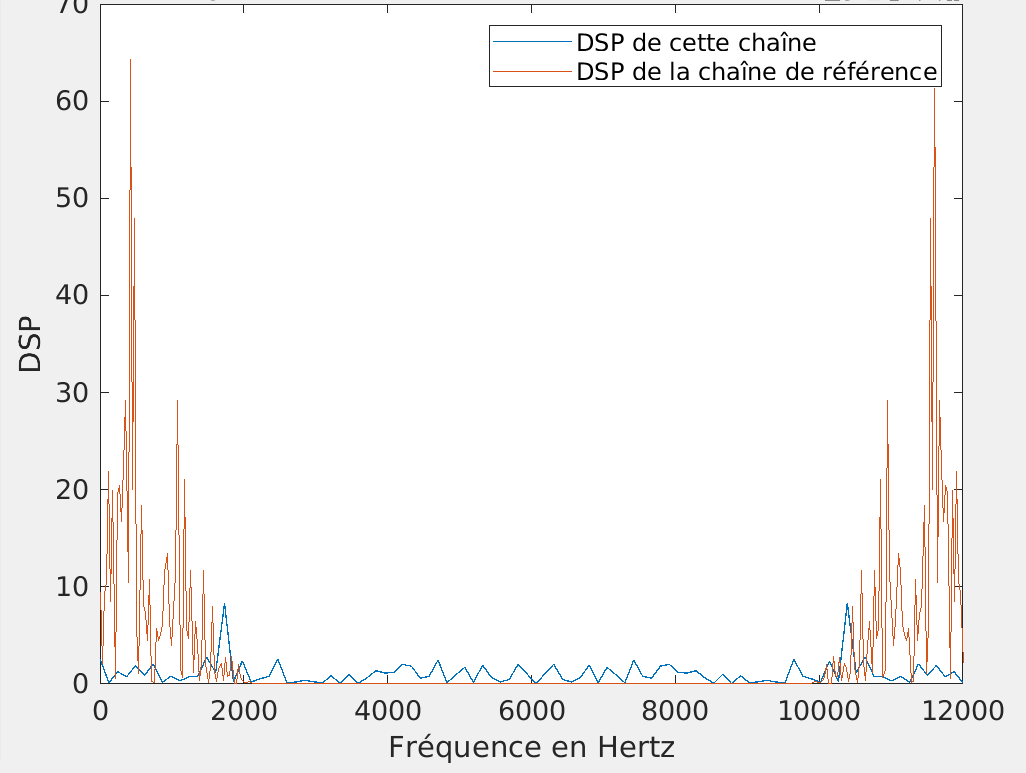
\includegraphics[width=7cm]{C3F52.png}		              	    \caption{DSPs de la chaîne 3 et de la chaîne de référence. \label{fig : C3F52}}
		\end{figure}
		\newpage
		La chaîne la plus efficace spectralement est celle dont la courbe de la DSP est telle qu'elle montre qu'un maximum de l'information est contenu dans une faible bande de fréquence. 
		
		Ici, la courbe de la chaîne étudiée est celle qui vérifie cela.
		
		Donc, la chaîne étudiée est la plus efficace spectralement.
		\par\leavevmode\par
        \item Reprendre à la chaine de transmission sans bruit et introduire un passage dans un canal de transmission
            \begin{enumerate}
                \item de bande $BW=1500$ Hz (implanté comme un filtre passe bas de fréquence de coupure $1500$ Hz : voir TPs et projet de traitement du signal).
                \par\leavevmode\par
                \setlength\parindent{0.5cm}
                La figure \ref{fig : C3F621} représente un diagramme de l'oeil en sortie du filtre de réception de la chaîne sans bruit, avec un filtre canal passe bas de fréquence de coupure $1500$ Hz.
                \begin{figure}[ht!]
				\centering
				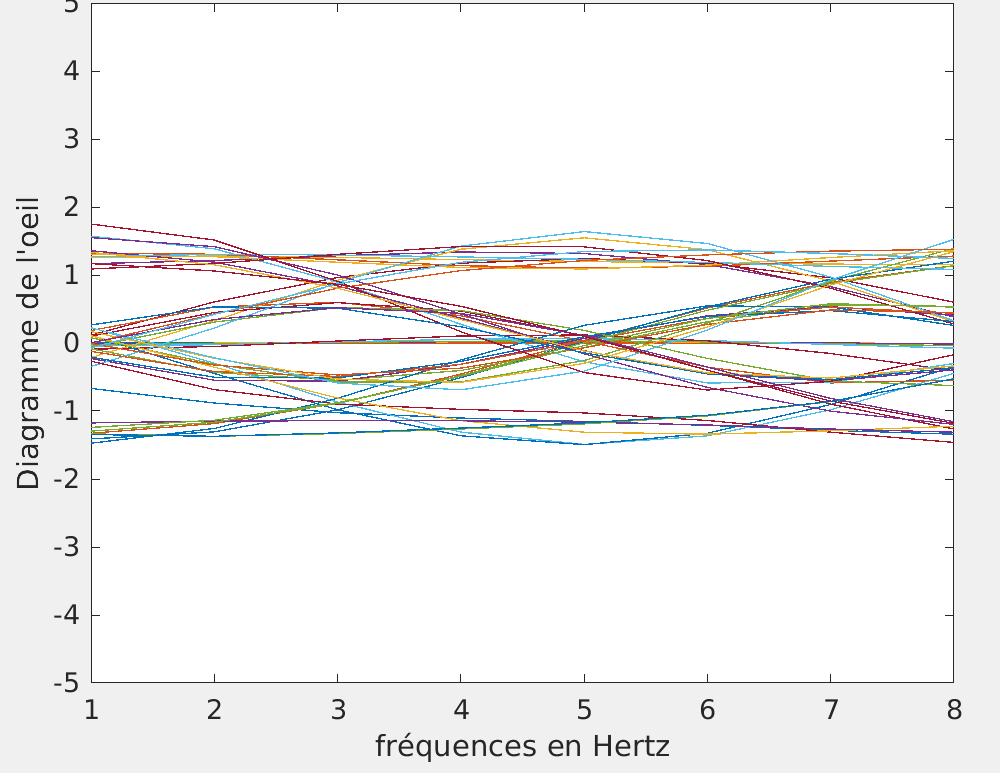
\includegraphics[width=8cm]{C3F621.png}		              	\caption{Diagramme de l'oeil en sortie du filtre de réception de la chaîne 3 sans bruit, avec un filtre canal passe bas de fréquence de coupure $1500$ Hz. \label{fig : C3F621}}
				\end{figure}
				\par\leavevmode\par
                \item de bande $BW=3000$ Hz (implanté comme un filtre passe bas de fréquence de coupure $3000$ Hz : voir TPs et projet de traitement du signal).
                \par\leavevmode\par
                \setlength\parindent{0.5cm}
                La figure \ref{fig : C3F622} représente un diagramme de l'oeil en sortie du filtre de réception de la chaîne sans bruit, avec un filtre canal passe bas de fréquence de coupure $3000$ Hz.
                \begin{figure}[ht!]
				\centering
				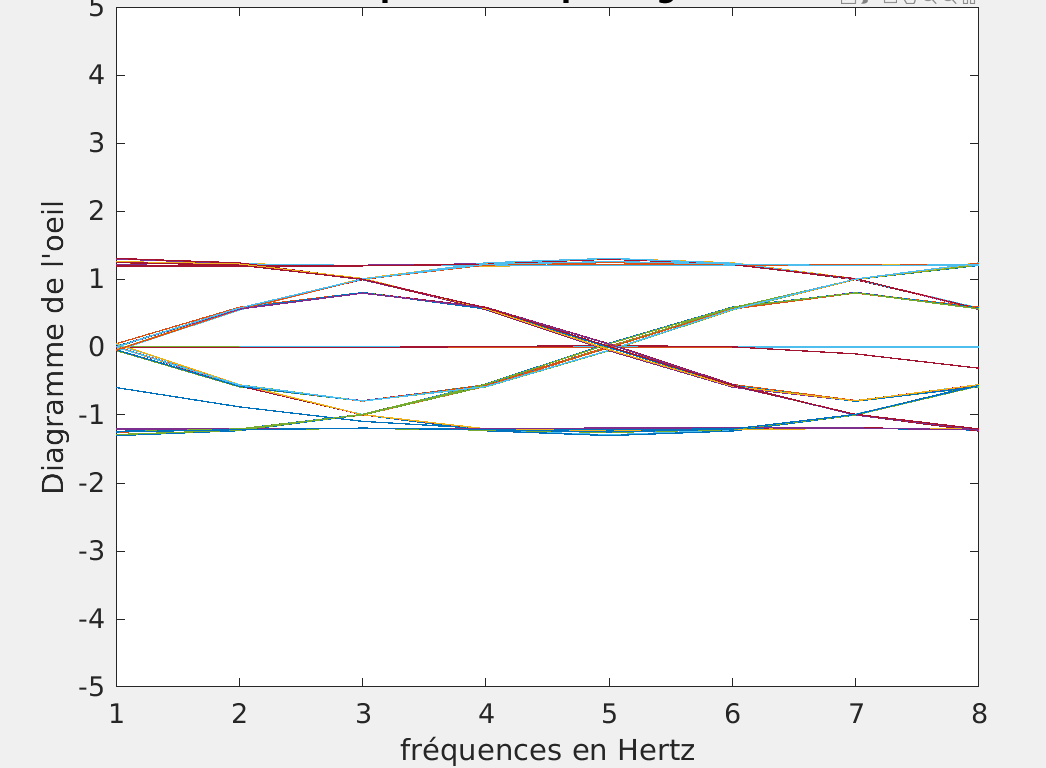
\includegraphics[width=8cm]{C3F622.png}		              	\caption{Diagramme de l'oeil en sortie du filtre de réception de la chaîne 3 sans bruit, avec un filtre canal passe bas de fréquence de coupure $3000$ Hz. \label{fig : C3F622}}
				\end{figure}
				\par\leavevmode\par
            \end{enumerate}
            Dans chaque cas tracer un diagramme de l'oeil en sortie du filtre de réception et expliquer les résultats obtenus, les différences observées. Sont-ils conformes avec votre étude théorique ?
            \par\leavevmode\par
            \setlength\parindent{0.5cm}
            Si on compare le diagramme de l'oeil avec $\text{BW} = 1500$ Hz avec celui réalisé sans passage du signal dans un canal, on observe qu'il n'est pas identique, contrairement à celui réalisé avec $\text{BW} = 3000$ Hz. En effet, dans ce dernier cas, toute l'information a été conservée, car le critère sur $R_s$ a été respecté.
            
            Théoriquement, afin de ne pas perdre d'information lors du filtrage, il faut que:
    $$R_s \leq \frac{2 \text{BW}}{(1 + \alpha)}$$
    
    Donc, $R_s$ doit vérifier:  
    $$ R_s \leq 2000 \; \text{pour BW} = 1500 \text{Hz} $$
    $$ R_s \leq 4000 \; \text{pour BW} = 3000 \text{Hz} $$
    
    Comme $R_s = 3000$ symboles par seconde, alors le filtre qu'il faudrait utiliser devrait être celui avec pour bande passante $\text{BW} = 3000$ Hz. 
            
    \end{enumerate}

%%%%%%%%%%%%%%%%%%%%%%%%%%%%%%%%%%%%%%%%%%%%%%%%%%%%%%%%%%%%%%%%%%
\section{Quatrième chaine à étudier : impact du choix du mapping}
%%%%%%%%%%%%%%%%%%%%%%%%%%%%%%%%%%%%%%%%%%%%%%%%%%%%%%%%%%%%%%%%%%
On considèrera un mapping $4$-aire à moyenne nulle (symboles $a_k \in \left\{-3, -1, 1, 3\right\}$) et des réponses impulsionnelles des filtres de mise en forme et de réception, $h(t$) et $h_r(t)$, rectangulaire de durée $Ts$.

\subsection{Etude théorique}

    \begin{enumerate}
        \item Proposer un instant optimal $t_0$ pour démarrer l'échantillonnage en expliquant votre choix. On échantillonnera alors aux instants optimaux $t_0+mT_s$, $m=0, 1, 2, ...$.
        \par\leavevmode\par
        \setlength\parindent{0.5cm}
        Comme les deux filtres sont rectangulaires de durée $T_s$, on se situe dans le même cas que pour la chaîne de réference en ce qui concerne la détermination des instants optimaux. 
        
        Ainsi, on prend comme instant optimal d'échantillonnage:
        $$
        \boxed{t_0 = T_s}
        $$
        
        \item En supposant que l'on utilise un détecteur à seuil pour prendre les décisions, quels sont les seuils optimaux à utiliser ? Justifiez votre réponse.
        
        \par\leavevmode\par
        \setlength\parindent{0.5cm}
        On a:
        
        $$a_k \in \left\{-3, -1, 1, 3\right\}$$
        
        En considérant la règle de décision du Maximum A Posteriori: 
         
        $$ \hat{a}_m = \underset{\tilde{a}_m}{\mathrm{argmax}} \mathbb{P}(\tilde{a}_m|z_m)$$
        
        Pour un mapping $4-aire$, on obtient la figure \ref{fig : 4_aire proba}: 
        
        \begin{figure}[ht!]
        \centering
        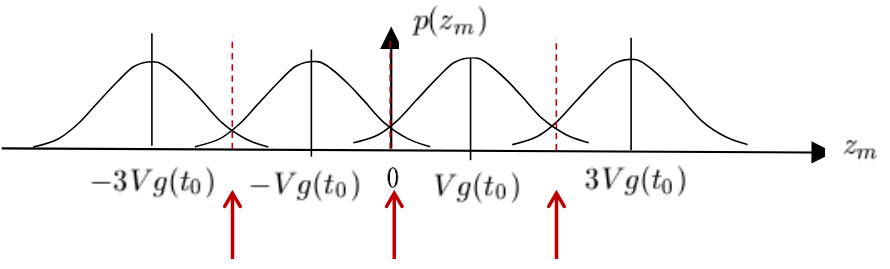
\includegraphics[width=10cm]{4_aire_proba.png}
        \caption{$\mathbb{P}(z_m)$ dans le cas $4-aire$ \label{fig : 4_aire proba}}
        \end{figure}
        
        On en déduit que les seuils optimaux sont: $-2 V g(t_0)$, $0$, et $2 V g(t_0)$, avec ici $V = 1$ et $g(t_0) = T_s$. 
        
        \item On suppose que l'on échantillonne aux instants optimaux et que l'on utilise un détecteur à seuil avec seuils optimaux. En utilisant le mapping suivant : $00: -3$,  $01: -1$, $11: +1$,  $10: +3$ :
                \begin{enumerate}
                    \item Calculer la probabilité de détecter (en sortie du bloc décision) le symbole $-1$ alors que l'on a émis $-3$.
                    
                    \begin{equation*}
                    \begin{split}                    
                    \mathbb{P}\left(\tilde{a}_m = -1 |a_m = -3\right) & = \mathbb{P}\left(-2 T_s \leq z_m \leq 0 | z_m = -3 T_s + \omega_m\right)\\
                    & = \mathbb{P}\left(-2 T_s \leq -3 T_s + \omega_m \leq 0\right) \\
                    & = \mathbb{P}\left(T_s \leq \omega_m \leq 3 T_s\right) \\
                    & = \mathbb{P}\left(\frac{T_s}{\sigma} \leq \frac{\omega_m}{\sigma} \leq \frac{3 T_s}{\sigma}\right) \\
                    & = - \mathbb{P}\left(\frac{\omega_m}{\sigma} > \frac{3 T_s}{\sigma} \right) + \mathbb{P}\left(\frac{\omega_m}{\sigma} > \frac{T_s}{\sigma} \right)\\
                    & = - Q\left(\frac{3 T_s}{\sigma} \right) + Q\left(\frac{T_s}{\sigma} \right)\\
                    \end{split}
                    \end{equation*}
                    $$\boxed{\mathbb{P}\left(\tilde{a}_m = -1 |a_m = -3\right) = - Q\left(\frac{3 T_s}{\sigma} \right) + Q\left(\frac{T_s}{\sigma} \right)}$$
                    \item Calculer la probabilité de détecter (en sortie du bloc décision) le symbole $+1$ alors que l'on a émis $-3$.
                    
                    \begin{equation*}
                    \begin{split}                    
                    \mathbb{P}\left(\tilde{a}_m = 1 |a_m = -3\right) & = \mathbb{P}\left(0 \leq z_m \leq 2 T_s | z_m = -3 T_s + \omega_m\right)\\
                    & = \mathbb{P}\left(0 \leq -3 T_s + \omega_m \leq 2 T_s\right) \\
                    & = \mathbb{P}\left(3 T_s \leq \omega_m \leq 5 T_s\right) \\
                    & = \mathbb{P}\left(\frac{3 T_s}{\sigma} \leq \frac{\omega_m}{\sigma} \leq \frac{5 T_s}{\sigma}\right) \\
                    & = - \mathbb{P}\left(\frac{\omega_m}{\sigma} > \frac{5 T_s}{\sigma} \right) + \mathbb{P}\left(\frac{\omega_m}{\sigma} > \frac{3 T_s}{\sigma} \right)\\
                    & = - Q\left(\frac{5 T_s}{\sigma} \right) + Q\left(\frac{3 T_s}{\sigma} \right)\\
                    \end{split}
                    \end{equation*}
                    $$\boxed{\mathbb{P}\left(\tilde{a}_m = -1 |a_m = -3\right) = - Q\left(\frac{5 T_s}{\sigma} \right) + Q\left(\frac{3 T_s}{\sigma} \right)}$$
                    \item Calculer la probabilité de détecter (en sortie du bloc décision) le symbole $+3$ alors que l'on a émis $-3$.
                    
                    \begin{equation*}
                    \begin{split}                    
                    \mathbb{P}\left(\tilde{a}_m = +3 |a_m = -3\right) & = \mathbb{P}\left(z_m \geq 2 T_s | z_m = -3 T_s + \omega_m\right)\\
                    & = \mathbb{P}\left(-3 T_s + \omega_m \geq 2 T_s\right) \\
                    & = \mathbb{P}\left(\omega_m \geq 5 T_s\right) \\
                    & = \mathbb{P}\left(\frac{\omega_m}{\sigma} \geq \frac{5 T_s}{\sigma}\right) \\
                    & = Q\left(\frac{5 T_s}{\sigma}\right)\\
                    \end{split}
                    \end{equation*}
                    $$ \boxed{\mathbb{P}\left(\tilde{a}_m = +3 |a_m = -3\right) = Q\left(\frac{5 T_s}{\sigma}\right)}$$
                    \item AN : $N_0=10^{-3} V^2/Hz$, $R_b=1$ kbps.
                    
                    D'après la définition de la puissance du bruit:
                    $$ P_{\omega} = \int_\mathbb{R}S_{\omega}(f) \ \mathrm{d}f$$
                    
                    D'après la formule de Wiener-Lee:
                    
                    $$ P_{\omega} = \int_{\mathbb{R}}|H_r(f)|^2 \frac{N_0}{2} \ \mathrm{d}f$$
                    
                    D'où:
                    
                    $$ \sigma = \sqrt{\frac{N_0 T_s}{2}} V$$
                    
                    De plus: 
                    \begin{equation*}
                    \begin{split}
                    R_s &= \frac{1}{2} R_b\\
                    T_s &= \frac{2}{R_b} \\
                    T_s &= 2 \mathrm{x}10^{-3} s \\
                    \sigma &= 1 \mathrm{x}10^{-3} V\\
                    \frac{T_s}{\sigma} &= 2 \ s V^{-1}\\
                    \end{split}
                    \end{equation*}
                    
                    Donc, à l'aide de la table de la fonction $Q$ de la loi normale centrée réduite:
                    
                    \begin{equation*}
                    \begin{split}
                    \mathbb{P}\left(\tilde{a}_m = -1 |a_m = -3\right) &\simeq 0.0228 \\
                    \mathbb{P}\left(\tilde{a}_m = 1 |a_m = -3\right) &\simeq 0\\
                    \mathbb{P}\left(\tilde{a}_m = 3 |a_m = -3\right) &\simeq 0 \\
                    \end{split}
                    \end{equation*}
                    
                    %\emph{La fonction $Q(x)=\frac{1}{\sqrt{2 \pi}}\int_x^{+ \infty} e^{-\frac{u^2}{2}}du$ est donnée par la figure \ref{Qfunc} en fin d'énoncé.}
                    \item La règle de codage choisie pour le mapping vous parait-elle intéressante ? Si oui, quel est son intérêt ?
                    
                    La règle de codage choisie pour le mapping suit le mapping de Gray. 
                    
                    Elle est intéressante car, pour passer d'un symbole à l'autre, seul un bit change à chaque fois.
                    
                    Ainsi, 
                    \begin{equation*}
                    \begin{split}
                    nb_{symboles faux} &\simeq nb_{bits faux} \\
                    TES & \simeq TEB \ log2(M)\\
                    \end{split}
                    \end{equation*}
                    \item Sachant que le taux d'erreur symbole de la chaîne est donné par :
                    $$
                    TES= \frac{3}{2}Q\left(\sqrt{\frac{4}{5}\frac{E_b}{N_0}}\right)
                    $$
                    Avec la règle de codage choisie pour le mapping donnez le taux d'erreur binaire (TEB) de la liaison, en expliquant votre réponse.
                    \begin{equation*}
                    \begin{split}
                    TEB & \simeq \frac{1}{log2(M)} \ TES\\
                    TEB & \simeq \frac{1}{2} \ TES\\
                    TEB & \simeq \frac{3}{4} \ Q\left(\sqrt{\frac{4}{5}\frac{E_b}{N_0}}\right)
                    \end{split}
                    \end{equation*}
                \end{enumerate}
    \end{enumerate}

\subsection{Implantation sous Matlab}
\begin{enumerate}
        \item Implantation de la chaine sans bruit : on l'implantera en utilisant le mapping suivant : $00: -3$,  $01: -1$, $10: +1$,  $11: +3$ (voir en annexe). Attention le mapping est différent de celui proposé dans l'étude théorique précédente.
            \begin{enumerate}
                \item Tracer le signal en sortie du filtre d'émission, ainsi que sa densité spectrale de puissance. Ces tracés sont-ils conformes à la théorie ?
                \par\leavevmode\par
                \setlength\parindent{0.5cm}
                La figure \ref{fig : C4F12} représente  le signal en sortie du filtre d'émission pour 100 bits.
        
                 \begin{figure}[ht!]
		         \centering
		         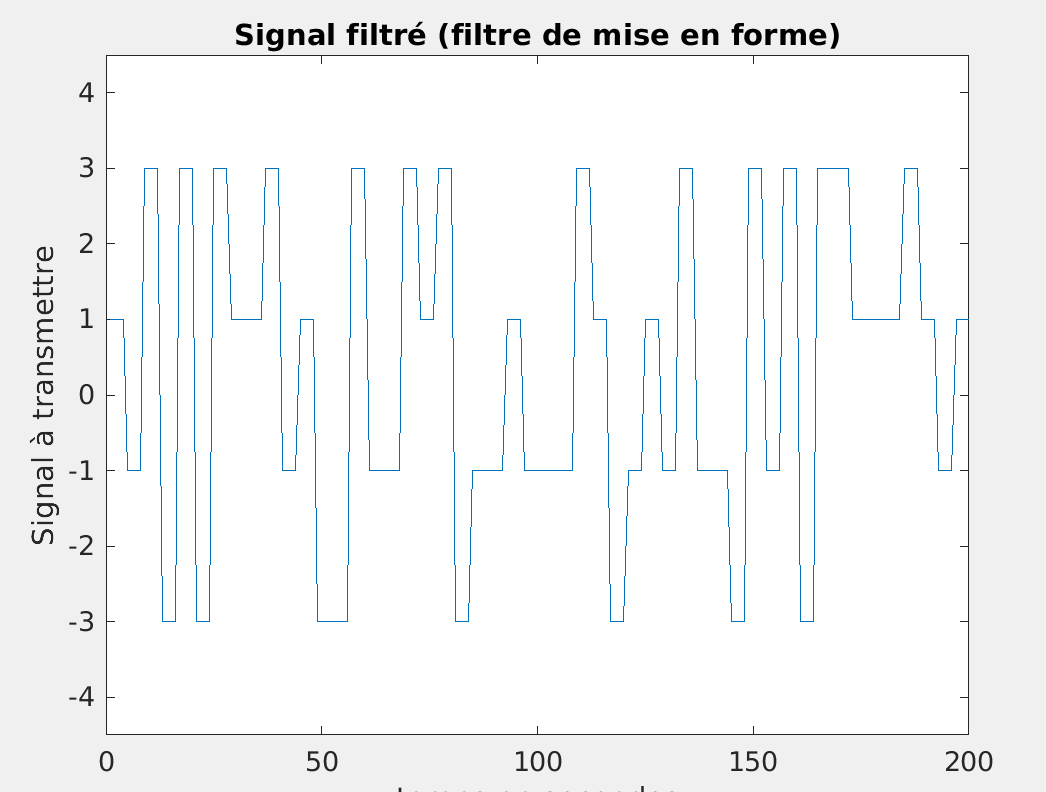
\includegraphics[width=10cm]{C4F12.png}		              			     \caption{Signal en sortie du filtre d'émission (100 bits transmis)(chaîne 4). \label{fig : C4F12}}
		         \end{figure}
		         
		        
		         \newpage
		         Le signal tracé après passage dans un filtre de mise en forme est conforme à l'étude théorique, c'est une somme de rectangles, un tous les $T_s$, pondérés par $3$, $1$, $-1$ ou $-3$.
		         
		         La figure \ref{fig : C4F22} représente la DSP du signal en sortie du filtre d'émission. 
		         
		         \begin{figure}[ht!]
		         \centering
		         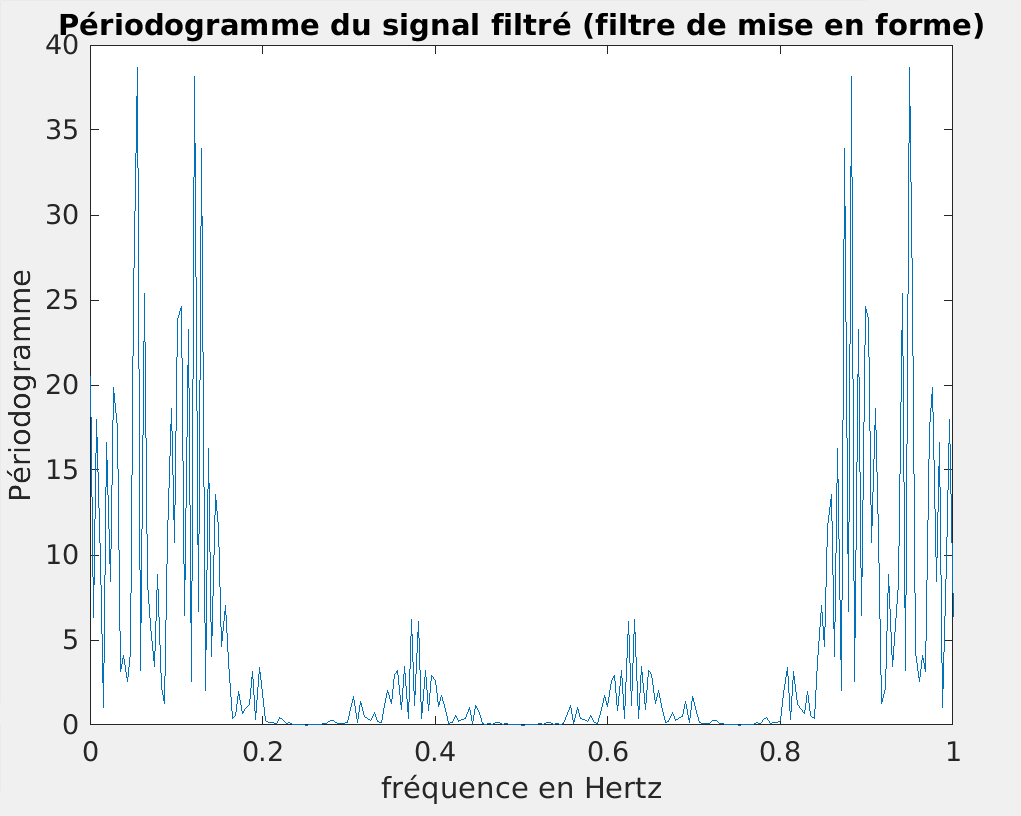
\includegraphics[width=10cm]{C4F22.png}		              	 \caption{DSP du signal en sortie du filtre d'émission(chaîne 4). \label{fig : C4F22}}
		         \end{figure}
		         
		         La DSP est aussi conforme à l'étude théorique car la DSP du signal est transmise autour de la fréquence $0$, elle est symétrique par rapport à l'axe des ordonnées, et une première annulation est présente à la fréquence $\frac{1}{T_s}$, soit $0,25$ Hz, une deuxième annulation est présente à la fréquence $\frac{2}{T_s}$, soit $0,5$ Hz.
		         \par\leavevmode\par
                \item Comparer l'efficacité spectrale de la chaine étudiée avec celle de la chaine de référence (en supperposant les tracés des DSPs des signaux transmis dans les deux cas pour un même débit binaire). La similitude ou différence obtenue devra être expliquée.La chaine éventuellement la plus efficace spectralement devra être identifiée, en expliquant pourquoi.
                \par\leavevmode\par
                \setlength\parindent{0.5cm}
                La figure \ref{fig : C4F32} représente les DSPs des signaux transmis pour cette chaîne et pour la chaîne de référence.  
		         
		         \begin{figure}[ht!]
		         \centering
		         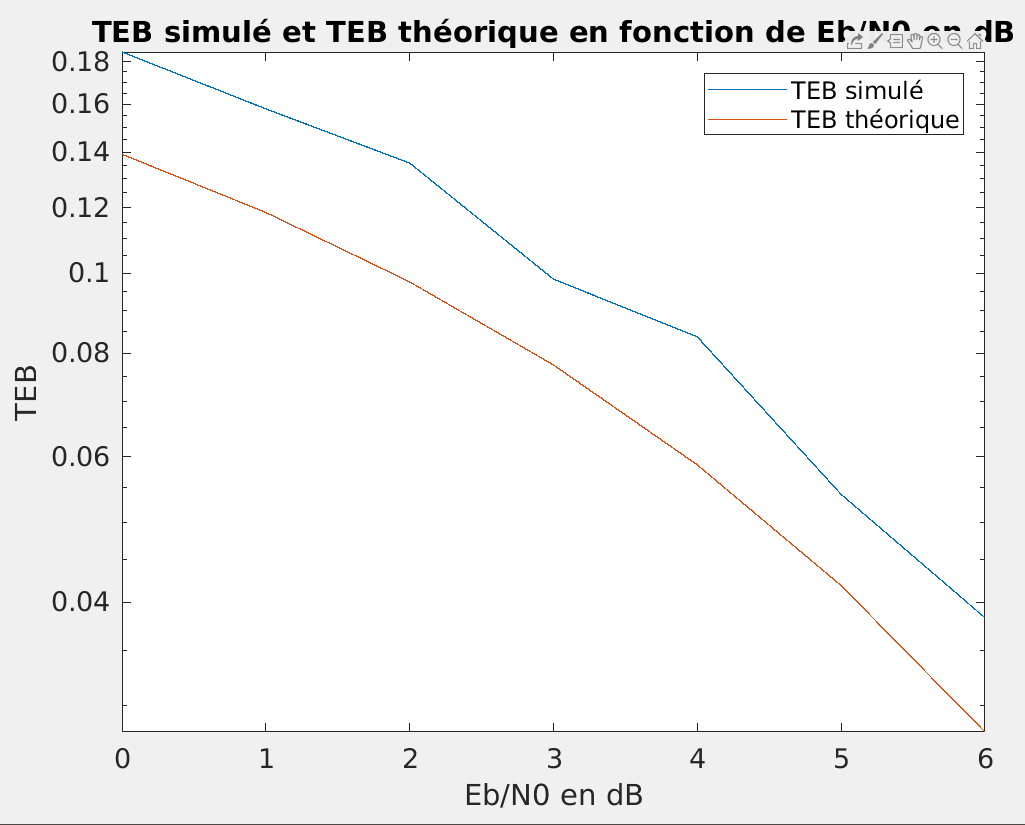
\includegraphics[width=10cm]{C4F32.png}		              	 \caption{DSP des signaux transmis pour cette chaîne et pour la chaîne de référence(chaîne 4). \label{fig : C4F32}}
		         \end{figure}
		         
		         Les zones où la DSP est non nulles et les zones d'annulations sont aux mêmes endroits, en revanche, l'amplitude des pics et leur étalement autour de la valeur du plus haut pic, varient d'une chaîne à l'autre, l'amplitude pour la chaîne étudiée étant beaucoup plus importante que pour la chaîne de réference. 
		         
		         Cela est dû au fait que les mêmes filtres sont utilisés, donc la forme globale est la même. Mais le mapping n'est pas le même, donc le poids de chaque fréquence n'est pas le même entre les deux chaînes.
		         
		         La chaîne la plus efficace spectralement est celle dont la courbe de la DSP est telle qu'elle montre qu'un maximum de l'information est contenu dans une faible bande de fréquence. 
		         
		         Ici, la courbe de la chaîne étudiée est celle qui vérifie cela.
		         
		         Donc, la chaîne étudiée est la plus efficace spectralement. 
				\par\leavevmode\par
                \item Tracer un diagramme de l'oeil en sortie du filtre de réception afin de déterminer les instants optimaux d'échantilllonnage et les seuils optimaux de décision (détecteur à seuil). Les résultats obtenus sont-ils conformes à la théorie ? Expliquez votre réponse.
                \par\leavevmode\par
       			 \setlength\parindent{0.5cm}
        		 La figure \ref{fig : C4F42} représente  un diagramme de l'oeil en sortie du filtre de réception.
        
                 \begin{figure}[ht!]
		         \centering
		         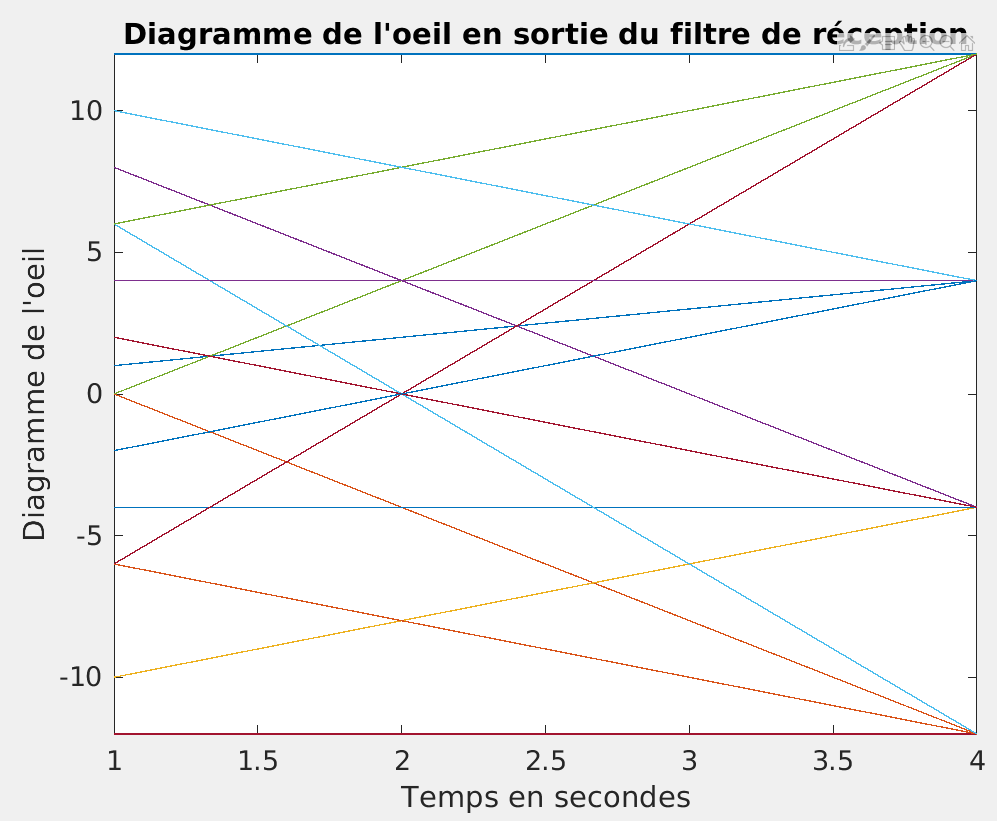
\includegraphics[width=8cm]{C4F42.png}		              	 \caption{Diagramme de l'oeil en sortie du filtre de réception (chaîne 4). \label{fig : C4F42}}
		         \end{figure}
		         
		        \newpage
		         L'amplitude des éléments du diagramme de l'oeil, lorsque le critère de Nyquist est respecté est de $a_m g(t_0)$, soit $a_m T_s$, soit $-12$, $-4$, $4$ et $12$ ($a_m \in \left\{-3, -1, 1, 3\right\}$, $T_s = 4$). Le seul endroit où une décision peut être prise est pour $t_0 = T_s$.
		         
		         On retrouve le résultat théorique : l'instant optimal d'échantillonnage est pour $t_0 = T_s$. 
		         \par\leavevmode\par 
		         
		         Les symboles tels que $a_m g(t_0)$ soit supérieur à $2 T_s = 8$, seront assignés à $3$, ceux tels que $a_m g(t_0)$ est inférieur à $-2 T_s = 8$ seront assignés à $-3$, ceux tels que $a_m g(t_0)$ soit compris entre $2 T_s$ et $0$ seront assignés à $1$, ceux tels que $a_m g(t_0))$ soit compris entre $-2 T_s$ et $0$ seront assignés à $-1$. 
		         
		         On retrouve les seuils théoriques qui sont $-2 T_s$, $0$ et $2 T_s$.
		         \par\leavevmode\par
                \item En utilisant les instants optimaux d'échantillonnage puis un détecteur à seuil, avec seuils optimaux, vérifier que le TEB obtenu est bien nul.
                
                \par\leavevmode\par
       			 \setlength\parindent{0.5cm}
       			 Avec $t_0 = T_s$ et un seuil à $0$, le TEB est bien nul. 
       			 \par\leavevmode\par
            \end{enumerate}
        \item Rajouter le bruit et tracer le taux d'erreur symbole (TES) obtenu en fonction du rapport signal à bruit par bit à l'entrée du récepteur ($E_b/N_0$) en décibels. On prendra des valeurs de $\left(E_b/N_0\right)_{dB}$ allant de $0$ à $6$ dB.
        
        \par\leavevmode\par
       	\setlength\parindent{0.5cm}
       	La figure \ref{fig : C4F72} représente le TES obtenu en fonction du rapport signal à bruit par bit à l'entrée du récepteur  ($\left(E_b/N_0\right)_{dB}$). 
        
        \begin{figure}[ht!]
		\centering
		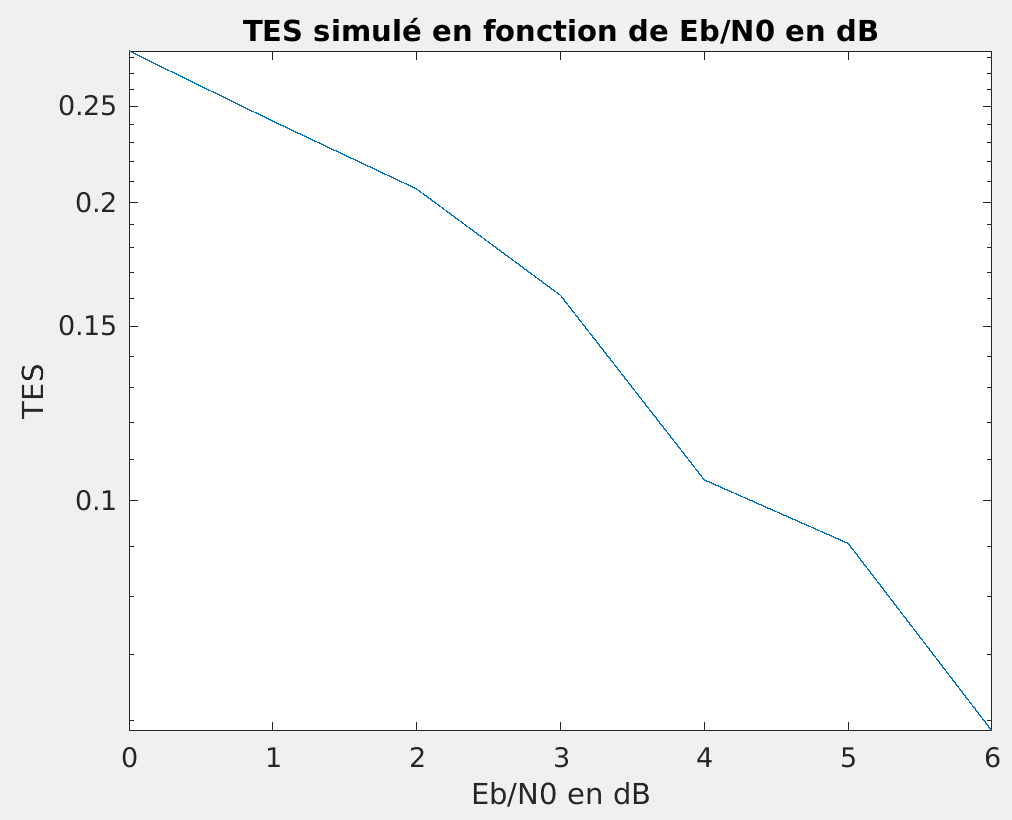
\includegraphics[width=8cm]{C4F72.png}		              	    \caption{TES obtenu en fonction de $\left(E_b/N_0\right)_{dB}$ (chaîne 4). \label{fig : C4F72}}
		\end{figure}
		
		\par\leavevmode\par
		\newpage
        \item Comparer le TES obtenu par simulation sur la chaine implantée au TES donné pour la chaine étudiée dans l'étude théorique. La similitude ou différence obtenue devra être expliquée.
        
        
       	\par\leavevmode\par
       	\setlength\parindent{0.5cm}
       	La figure \ref{fig : C4F92} représente le TES simulé et le TES théorique en fonction du rapport signal à bruit par bit à l'entrée du récepteur  ($\left(E_b/N_0\right)_{dB}$). 
       	   
        \begin{figure}[ht!]
		\centering
		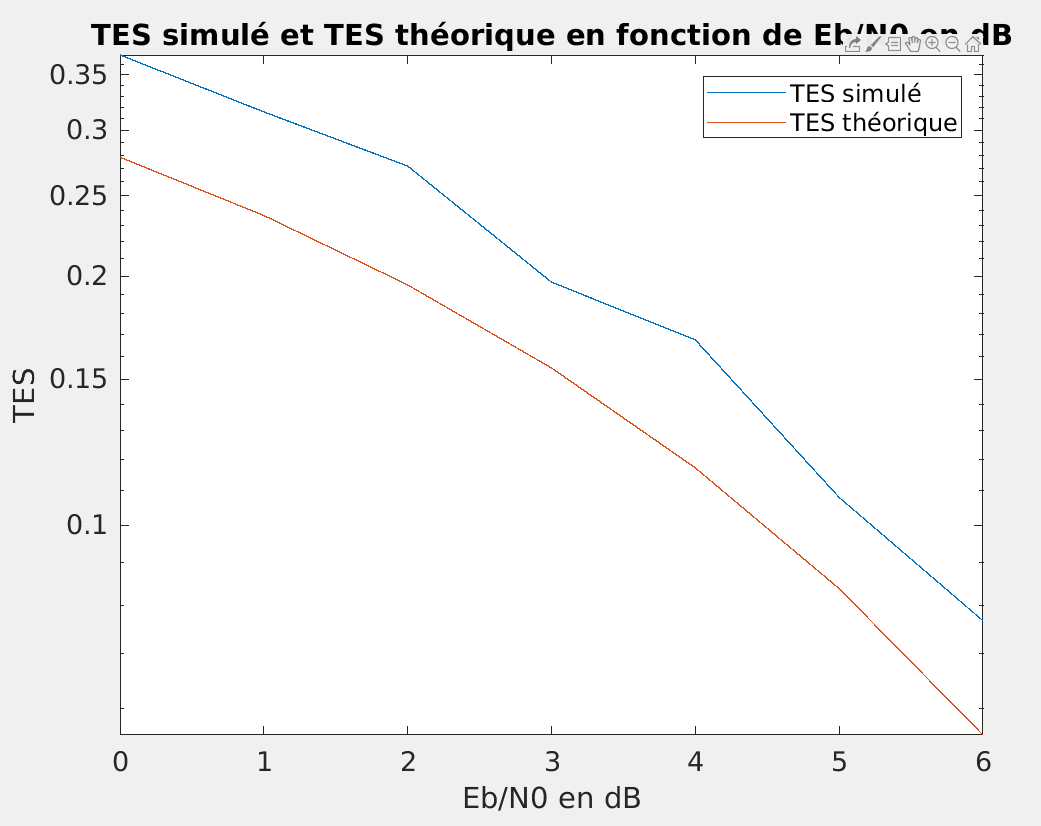
\includegraphics[width=8cm]{C4F92.png}		              	    \caption{TES simulé et le TES théorique en fonction de $\left(E_b/N_0\right)_{dB}$ (chaîne 4). \label{fig : C4F92}}
		\end{figure}
		
	
		
        \item Tracer le taux d'erreur binaire (TEB) obtenu en fonction du rapport signal à bruit par bit à l'entrée du récepteur ($E_b/N_0$) en décibels. On prendra des valeurs de $\left(E_b/N_0\right)_{dB}$ allant de $0$ à $6$ dB.
        \par\leavevmode\par
       	\setlength\parindent{0.5cm}
       	La figure \ref{fig : C4F82} représente le TEB obtenu en fonction du rapport signal à bruit par bit à l'entrée du récepteur  ($\left(E_b/N_0\right)_{dB}$). 
        
        \begin{figure}[ht!]
		\centering
		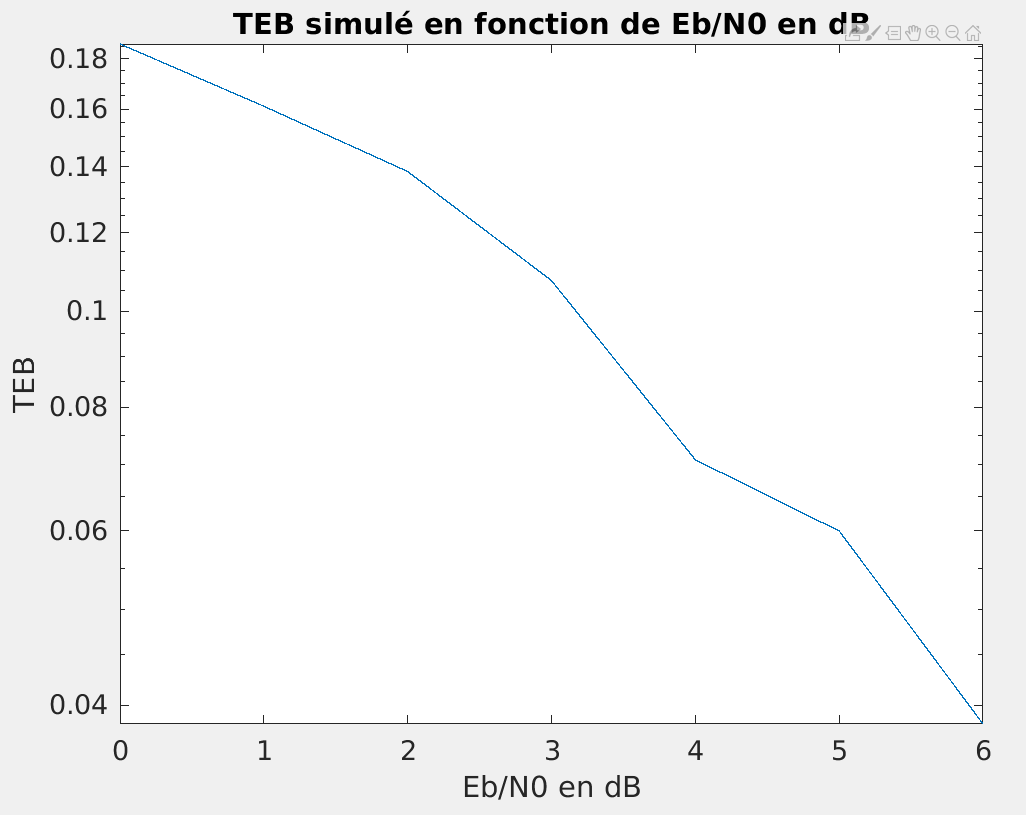
\includegraphics[width=8cm]{C4F82.png}		              	    \caption{TEB obtenu en fonction de $\left(E_b/N_0\right)_{dB}$ (chaîne 4). \label{fig : C4F82}}
		\end{figure}
		
		\par\leavevmode\par
		\newpage
        \item Comparer le TEB obtenu par simulation sur la chaine implantée au TEB donné pour la chaine étudiée dans l'étude théorique. La similitude ou différence obtenue devra être expliquée. La chaine éventuellement la plus efficace en puissance devra être identifiée, en expliquant pourquoi.
        \par\leavevmode\par
       	\setlength\parindent{0.5cm}
       	La figure \ref{fig : C4F32} représente le TEB simulé et le TEB théorique en fonction du rapport signal à bruit par bit à l'entrée du récepteur  ($\left(E_b/N_0\right)_{dB}$). 
       	 
        \begin{figure}[ht!]
		\centering
		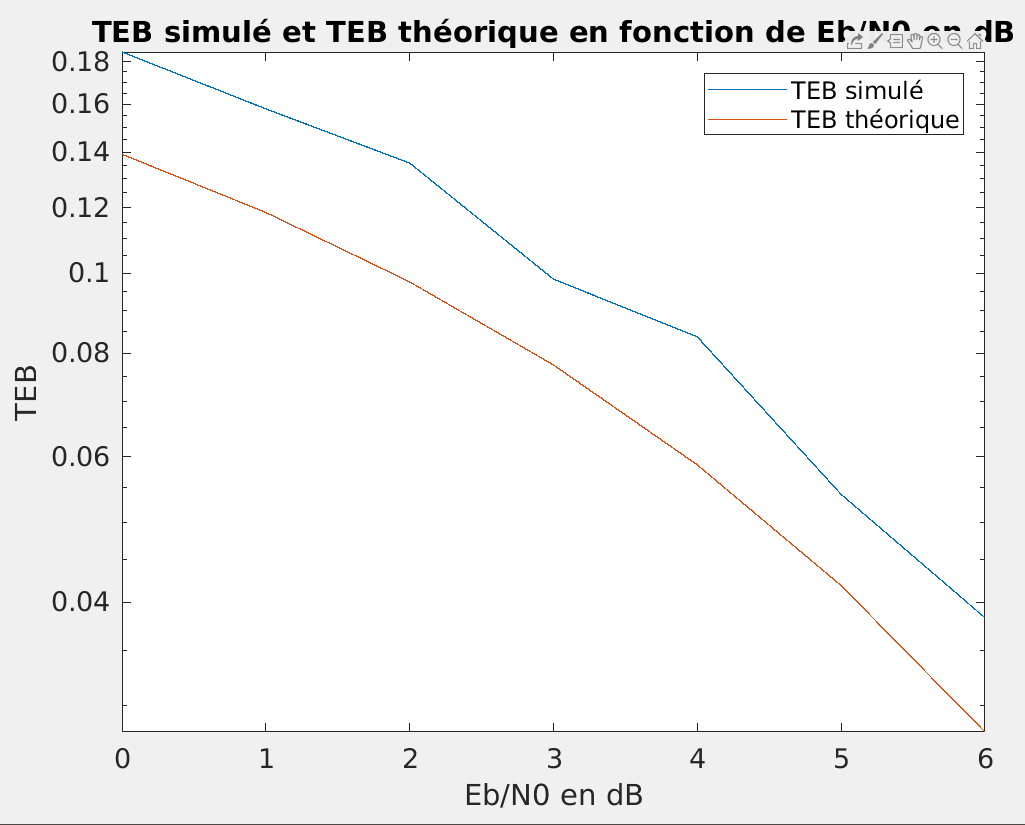
\includegraphics[width=8cm]{C4F32.png}		              	    \caption{TEB simulé et le TEB théorique en fonction de $\left(E_b/N_0\right)_{dB}$ (chaîne 4). \label{fig : C4F32}}
		\end{figure}
    \end{enumerate}
    
    Comme $\frac{4 E_b}{5 N_0} < \frac{2 E_b}{N_0}$, la courbe de TEB simulé de cette chaîne se situera au dessus de la courbe de TEB simulé de la chaîne de référence (par décroissance de la fonction Q). La chaîne de référence sera plus efficace spectralement. 

\section{Conclusion}
Le filtre de réception a une influence sur l'efficacité en puissance.

Le filtre de mise en forme a une influence sur l'efficacité spectrale, et le passage dans un canal, selon la bande passante considérée, peut induire une mauvaise transmission du message.

Augmenter le nombre de bits du mapping a un impact sur l'efficacité en puissance et spectrale, en effet cela permet d'améliorer l'efficacité spectrale et d'amoindrir l'efficacité en puissance. 

\section{Références}
\begin{enumerate}
	\item Cours
	\item TDs
	\item TPs
\end{enumerate}

\end{document}
